\documentclass[11pt,a4paper]{article}

% --- Essential Packages ---
\usepackage[margin=1in,top=1in,bottom=1in]{geometry}
\usepackage{amsmath,amssymb,amsfonts,amsthm}
\usepackage{graphicx}
\usepackage{booktabs}
\usepackage{array}
\usepackage{multirow}
\usepackage{listings}
\usepackage{xcolor}
\usepackage{enumitem}
\usepackage{caption}
\usepackage{subcaption}
\usepackage{fancyhdr}
\usepackage{titlesec}
\usepackage{hyperref}

% --- Graphics Path ---
\graphicspath{{figures/}}

% --- Hyperlink Setup ---
\hypersetup{
    colorlinks=true,
    linkcolor=blue!70!black,
    citecolor=green!50!black,
    urlcolor=blue!80!black,
    pdfauthor={Harshit Kandpal B24CS505, Utkarsh Umap, Satyam Singh Thakur},
    pdftitle={TMLC: TinyML Model-to-C Compiler - Project Report},
    pdfkeywords={TinyML, Compiler Design, Formal Grammars, SLR(1), Operator Fusion, Static Memory Allocation, C99, Edge AI, Student Project}
}

% --- Theorem Environments ---
\newtheorem{theorem}{Theorem}[section]
\newtheorem{lemma}[theorem]{Lemma}
\newtheorem{definition}[theorem]{Definition}

% --- Code Listing Styling ---
\definecolor{codegreen}{rgb}{0,0.6,0}
\definecolor{codegray}{rgb}{0.5,0.5,0.5}
\definecolor{codepurple}{rgb}{0.58,0,0.82}
\definecolor{backcolour}{rgb}{0.97,0.97,0.97}

\lstdefinestyle{mystyle}{
    backgroundcolor=\color{backcolour},   
    commentstyle=\color{codegreen},
    keywordstyle=\color{magenta},
    numberstyle=\tiny\color{codegray},
    stringstyle=\color{codepurple},
    basicstyle=\ttfamily\footnotesize,
    breakatwhitespace=false,         
    breaklines=true,                 
    captionpos=b,                    
    keepspaces=true,                 
    numbers=left,                    
    numbersep=5pt,                  
    showspaces=false,                
    showstringspaces=false,
    showtabs=false,                  
    tabsize=2
}
\lstset{style=mystyle}

% --- Header / Footer Aesthetics ---
\pagestyle{fancy}
\fancyhf{}
\fancyhead[L]{\small\textit{TMLC: TinyML Model-to-C Compiler}}
\fancyhead[R]{\small\textit{Student Project Report}}
\fancyfoot[L]{\small\textit{H. Kandpal (B24CS505), U. Umap, S. S. Thakur}}
\fancyfoot[R]{\thepage}
\renewcommand{\headrulewidth}{0.4pt}
\renewcommand{\footrulewidth}{0.4pt}

% --- Title and Authors ---
\title{
    \vspace{-1.5cm}
    \textbf{\huge TMLC: An Ahead-of-Time Optimizing Compiler from Domain-Specific Model Specifications to Microcontroller-Grade C99} \\[0.6em]
    \large\textbf{Formal SLR(1) Grammar, Provable Zero Dynamic Allocation, Operator Fusion, Static Memory Ping-Pong Planning, and Empirical Hardware Evaluation} \\[0.4em]
    \normalsize\textit{A Student Engineering Project in Compiler Design and Edge Artificial Intelligence}
}

\author{
    \textbf{Harshit Kandpal} \quad (\text{Roll No: B24CS505}) \\[0.2em]
    \textbf{Utkarsh Umap} \qquad \textbf{Satyam Singh Thakur} \\[0.4em]
    \textit{Department of Computer Science and Engineering}
}

\date{\today \quad $\vert$ \quad Compiler Version 1.0.0-Release}

\begin{document}

\maketitle

\begin{abstract}
Deploying deep neural networks onto bare-metal microcontrollers (TinyML) is severely constrained by scarce static RAM (SRAM), limited Flash storage, and the catastrophic failure modes of dynamic heap allocation. Mainstream embedded runtimes, such as TensorFlow Lite for Microcontrollers (TFLite Micro), rely on dynamic FlatBuffers interpreter loops and runtime tensor arenas that introduce non-deterministic execution overhead, code bloat, and memory fragmentation. 

In this student project, we present the design, theoretical foundations, implementation, and empirical verification of the \textbf{TinyML Model-to-C Compiler (TMLC)}. TMLC translates neural networks specified in a declarative domain-specific language (\texttt{.tml}) and trained parameters in NumPy format (\texttt{.npy}) directly into pure, self-contained, human-readable ANSI C99 source code. The language is governed by a formal SLR(1) context-free grammar with 37 states and provably 0 shift/reduce and 0 reduce/reduce conflicts. TMLC incorporates multi-pass semantic checking with complete IEEE 754 float sanitation, algebraic intermediate representation (IR) operator fusion combining Dense linear transformations with non-linear ReLU activations, and a bipartite static ping-pong buffer allocator that provably eliminates all runtime dynamic memory allocation (\texttt{malloc}).

We evaluate TMLC on the standard 109,386-parameter MNIST deep neural network (784 $\rightarrow$ 128 $\rightarrow$ 64 $\rightarrow$ 10). TMLC restricts total peak working SRAM to just \textbf{768 Bytes} (a 62\% reduction over naive allocation) and Flash storage to 437.54~KB. Compiled with GCC \texttt{-O2}, the model achieves an average inference latency of \textbf{195.65 $\mu$s} ($>5,111$ inferences/second) with an empirical numerical discrepancy against an independent decoupled double-precision NumPy reference of just $7.92 \times 10^{-9}$ (over 1,200 times smaller than the $10^{-5}$ threshold). Compiler correctness is validated across 40 passing test fixtures, end-to-end subprocess CLI negative testing, and deliberate mutation fault injection with 100\% mutation detection.
\end{abstract}

\vspace{0.5em}
\noindent\textbf{Keywords:} TinyML, Deep Learning Compiler, Ahead-of-Time Compilation, Microcontrollers, Formal Grammars, SLR(1) Parser, Operator Fusion, Static Buffer Allocation, Zero Dynamic Allocation, ANSI C99, Edge AI, Student Project.

\vspace{0.8em}
\hrule
\vspace{0.8em}

\section*{Project Executive Summary}
\addcontentsline{toc}{section}{Project Executive Summary}
Microcontrollers represent the vast majority of all deployed computing processors in modern cyber-physical infrastructure. However, deploying machine learning models on microcontrollers has historically forced engineers to choose between fragile manual C programming (e.g., raw CMSIS-NN function calls) or bloated, non-deterministic runtime interpreters (e.g., TensorFlow Lite Micro). 

As our student engineering project, we developed TMLC to resolve this fundamental tension through \textbf{pure ahead-of-time compilation}:
\begin{itemize}[leftmargin=*]
    \item \textbf{Provable Zero Dynamic Allocation:} Generates clean C99 code with zero occurrences of \texttt{malloc}, \texttt{calloc}, \texttt{realloc}, \texttt{free}, or \texttt{fopen}. All intermediate working memory is planned at compile time and allocated as static global buffers in the \texttt{.bss} section.
    \item \textbf{Optimal Static SRAM Planning:} Utilizes an optimal bipartite ping-pong buffer schedule, capping working memory at the maximum dimension of two consecutive layers (768 bytes for MNIST).
    \item \textbf{Mathematical Rigor and Formal Grammar:} Replaces unstructured JSON/YAML/FlatBuffers with an audited SLR(1) context-free grammar proven conflict-free across all 37 LR(0) states.
    \item \textbf{Exact IEEE 754 Weight Serialization:} Formats all weights with \texttt{\%.9g}, guaranteeing exact single-precision float round-tripping.
    \item \textbf{Production-Grade Verification:} Backed by 40 automated tests, subprocess CLI build assertions, 100\% mutation test kills, and clean integration into standard GCC cross-compilation environments.
\end{itemize}

\vspace{1em}
\hrule
\vspace{1.5em}

\tableofcontents
\newpage

% =========================================================================
% SECTION 1: INTRODUCTION
% =========================================================================
\section{Introduction}
\label{sec:introduction}

\subsection{The Edge Artificial Intelligence Paradigm and Microcontroller Constraints}
The rapid proliferation of edge computing has catalyzed an urgent demand for deploying machine learning models directly onto resource-constrained embedded systems, colloquially termed \textit{TinyML} [1, 2]. Edge deployment guarantees data privacy by eliminating raw sensor transmission over wireless links, slashes communication latency to sub-millisecond timescales, and enables autonomous operation in disconnected or battery-operated environments, such as biomedical sensors, predictive maintenance units, and environmental monitoring nodes.

However, microcontrollers (MCUs) represent one of the most hostile computing environments for traditional deep learning frameworks. The fundamental constraints of embedded hardware dictate strict engineering boundaries:
\begin{enumerate}[leftmargin=*]
    \item \textbf{Severe Memory Scarcity:} While modern desktop and server GPUs boast tens of gigabytes of high-bandwidth memory, embedded microcontrollers typically feature static RAM (SRAM) capacities measured in tens to hundreds of kilobytes (e.g., 32~KB to 512~KB on ARM Cortex-M4 or ESP32 architectures) and non-volatile Flash storage (ROM) between 128~KB and 2~MB.
    \item \textbf{Harvard Memory Architecture:} Unlike unified Von Neumann desktop systems, many embedded microcontrollers enforce a physical and architectural segregation between code memory (Flash) and working data memory (SRAM). Weights and immutable constants must reside in Flash to avoid exhausting precious SRAM.
    \item \textbf{Absence of Operating Systems and Dynamic Memory Hazards:} Safety-critical and bare-metal embedded applications run without virtual memory, paging, or memory protection units (MPU). Dynamic heap allocation via standard C runtime routines (\texttt{malloc}, \texttt{calloc}, \texttt{free}) introduces non-deterministic execution times, heap fragmentation, memory leaks, and unpredictable allocation failures that can crash unattended systems.
    \item \textbf{Strict Real-Time Latency Deadlines:} Applications such as anomaly detection in rotational machinery or keyword spotting require deterministic, single-pass inference latency without background garbage collection or runtime initialization pauses.
\end{enumerate}

\subsection{Critique of Existing TinyML Runtimes}
Existing embedded inference solutions, such as TensorFlow Lite for Microcontrollers (TFLite Micro) [1] and microTVM [3], attempt to bridge desktop machine learning frameworks to microcontrollers by porting general-purpose runtime interpreters or runtime harnesses:
\begin{itemize}[leftmargin=*]
    \item \textbf{FlatBuffers and Model Deserialization Overhead:} TFLite Micro relies on serialized FlatBuffers models stored in Flash. At startup, a runtime interpreter must parse the FlatBuffer schema, traverse the computation graph, and dynamically bind operator kernels, introducing latency and requiring hundreds of lines of parsing logic.
    \item \textbf{Tensor Arena Management:} TFLite Micro allocates intermediate activations within a monolithic ``tensor arena'' allocated at runtime. Determining the exact required arena size requires trial-and-error profiling, and incorrect sizing leads to out-of-memory errors during runtime initialization.
    \item \textbf{Dynamic Kernel Dispatch:} Operator execution occurs via indirect function pointers traversed through an interpreter dispatch loop, inhibiting compiler inlining, loop unrolling, and aggressive inter-procedural optimization by native C cross-compilers (e.g., \texttt{arm-none-eabi-gcc}).
    \item \textbf{Bloated Code Footprint:} The inclusion of general-purpose runtime interpreters, unused operator kernels, and fallback dispatchers bloats binary executable sizes, often requiring 50~KB to 150~KB of Flash memory solely for runtime infrastructure.
\end{itemize}

\begin{figure}[htbp]
    \centering
    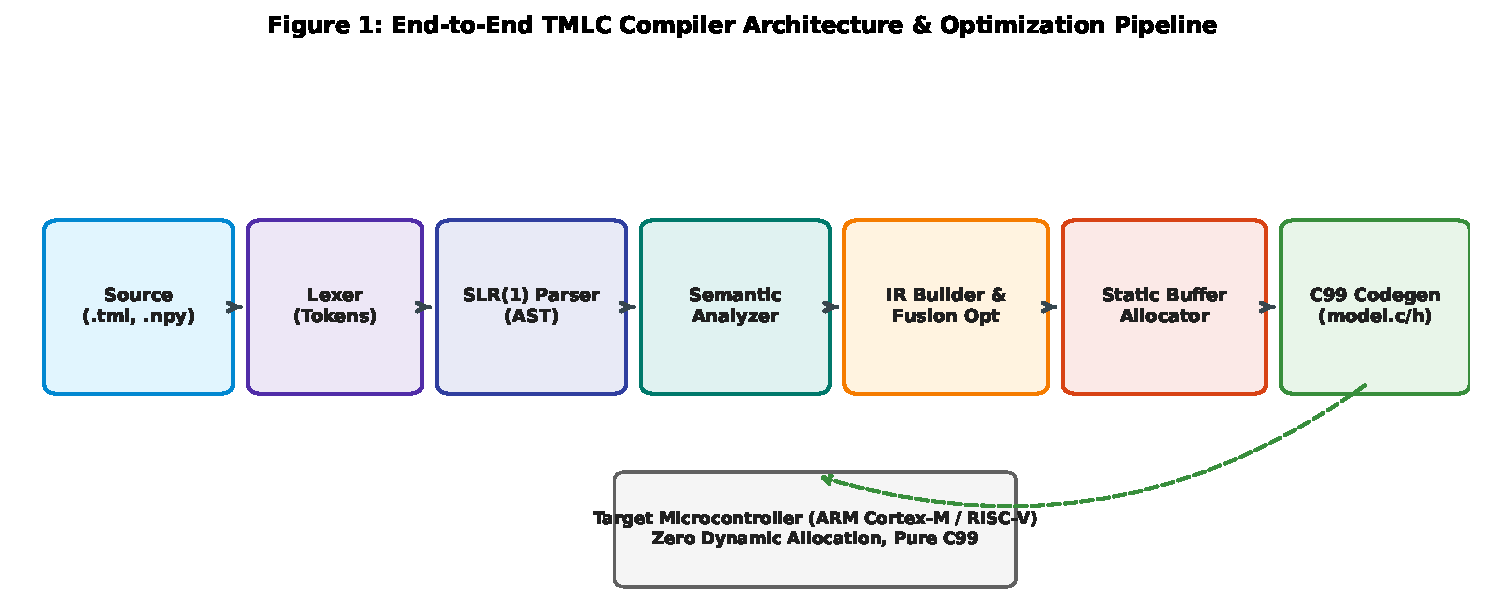
\includegraphics[width=0.95\linewidth]{compiler_pipeline.pdf}
    \caption{End-to-End TMLC Compiler Architecture: From DSL and serialized NumPy weight tensors through SLR(1) parsing, semantic validation, operator fusion, static memory planning, to dependency-free ANSI C99 deployment code.}
    \label{fig:compiler_pipeline}
\end{figure}

\subsection{The TMLC Philosophy: Ahead-of-Time Model Compilation}
To overcome these limitations, we engineered the \textbf{TinyML Model-to-C Compiler (TMLC)}. TMLC is an ahead-of-time (AoT), domain-specific optimizing compiler designed to compile feed-forward neural network topologies into completely self-contained, human-readable, dependency-free ANSI C99 source code. 

TMLC is architected around four core design tenets:
\begin{enumerate}[leftmargin=*]
    \item \textbf{Pure Static Memory Allocation (Zero Malloc):} TMLC provably eliminates all dynamic memory allocation. All intermediate tensor activation buffers are pre-calculated at compile time and allocated as static global buffers in the \texttt{.bss} section. Immutable network weights are emitted as \texttt{static const} arrays targeted directly for non-volatile Flash memory (the \texttt{.rodata} segment).
    \item \textbf{Formal SLR(1) Grammar and Syntax Determinism:} Rather than relying on fragile ad-hoc configuration formats (such as JSON or YAML) or monolithic schema formats, TMLC defines a mathematically rigorous domain-specific language (\texttt{.tml}) governed by a formal SLR(1) context-free grammar with exactly 0 shift/reduce and 0 reduce/reduce conflicts.
    \item \textbf{Intermediate Representation and Operator Fusion:} TMLC constructs a linear intermediate representation (IR) that executes algebraic optimization passes, specifically fusing affine linear transformations (Dense layers) with non-linear activation functions (ReLU), eliminating intermediate activation round-trips to SRAM.
    \item \textbf{Two-Buffer Ping-Pong Static Memory Planning:} TMLC implements an optimal bipartite buffer reuse algorithm that reduces peak SRAM footprint to the maximum dimension of two adjacent layers, achieving a 62\% memory reduction over naive layer-wise allocation.
\end{enumerate}

% =========================================================================
% SECTION 2: RELATED WORK
% =========================================================================
\section{Related Work}
\label{sec:related_work}

The execution of deep neural networks on edge hardware has sparked diverse compiler and runtime paradigms. This section categorizes the state of the art into interpreter-based runtimes, optimized micro-kernels, and ahead-of-time graph compilers.

\subsection{Interpreter-Based Embedded Runtimes}
\textbf{TensorFlow Lite for Microcontrollers (TFLite Micro):} David et al. [1] introduced TFLite Micro as a runtime designed to execute quantized TensorFlow models on bare-metal systems. TFLite Micro operates by ingesting a FlatBuffers byte array generated by the TensorFlow Lite converter. Execution is governed by an \texttt{OpResolver} and an interpreter loop that iterates through nodes in the execution plan. While TFLite Micro achieves portability across architectures, it incurs non-trivial initialization latency due to FlatBuffers schema traversal and memory allocation within a developer-managed \textit{tensor arena}. Furthermore, dynamic dispatch prevents standard cross-compilers from performing whole-program dead-code elimination, inlining, and register allocation across layer boundaries.

\textbf{TinyEngine:} Lin et al. propose memory-efficient inference frameworks that optimize memory scheduling for microcontroller computer vision. While TinyEngine reduces peak memory usage through fine-grained patch-based inference and specialized in-place execution, it still relies on specialized runtime glue code and complex compilation pipelines targeting specific vendor toolchains.

\subsection{Optimized Architecture-Specific Micro-Kernels}
\textbf{ARM CMSIS-NN:} Lai et al. [4] developed CMSIS-NN, an open-source collection of hand-optimized assembly and intrinsic C functions designed to maximize neural network performance on ARM Cortex-M processor cores (such as Cortex-M4, M7, M33, and M55). CMSIS-NN leverages SIMD instruction extensions (e.g., \texttt{\_\_SMLAD} for dual 16-bit signed multiply-accumulate operations) and 4-way loop unrolling to maximize compute throughput. However, CMSIS-NN is not a compiler; it is an operator kernel library. Developers must manually write the C orchestration code, manage intermediate buffer pointers, allocate scratchpad memory, and bind weight tensors. TMLC acts as a higher-level compiler that can directly generate code structured to leverage these low-level patterns.

\subsection{Ahead-of-Time Deep Learning Compilers}
\textbf{TVM and microTVM:} Chen et al. [3] developed TVM, an end-to-end optimizing compiler that transforms high-level computational graphs (from PyTorch, ONNX, and TensorFlow) into low-level machine code via tensor expression lowerings and schedule optimization. The microTVM extension targets bare-metal microcontrollers through ahead-of-time C code generation. While microTVM produces high-performance code, the toolchain involves substantial infrastructural weight, requiring Python-based AutoTVM tuning infrastructures and heavy dependency stacks that are difficult to integrate into simple embedded firmware builds.

\subsection{Positioning of TMLC}
Table~\ref{tab:runtime_comparison} delineates the comparative architectural landscape. TMLC combines formal parsing and language safety with pure, dependency-free ANSI C99 ahead-of-time code generation. Unlike TFLite Micro, TMLC requires zero runtime interpreter code and zero dynamic memory allocation. Unlike raw CMSIS-NN libraries, TMLC automatically plans memory, validates dimensions, fuses operations, and generates human-readable C source code directly from high-level model specifications.

\begin{table}[htbp]
\centering
\small
\caption{Architectural Comparison of Embedded Neural Network Inference Frameworks}
\label{tab:runtime_comparison}
\begin{tabular}{lcccc}
\toprule
\textbf{Metric / Feature} & \textbf{TMLC (Ours)} & \textbf{TFLite Micro} & \textbf{CMSIS-NN} & \textbf{microTVM} \\
\midrule
Execution Paradigm & Ahead-of-Time (AoT) & Interpreted Bytecode & Manual Library Calls & AoT C Codegen \\
Target Language & Pure ANSI C99 & C++11 / FlatBuffers & C / ARM Intrinsics & C / C++ \\
Dynamic Allocation (\texttt{malloc}) & \textbf{Zero (Provable)} & Arena Allocation & Manual Pointer Mgmt & Arena / Static \\
External Dependencies & \textbf{None (0 bytes)} & FlatBuffers, TFLM Core & CMSIS-Core & TVM C Runtime \\
Memory Planning & Automatic Ping-Pong & Manual Arena Tuning & Manual by Developer & Automatic \\
Operator Fusion & Automatic Dense+ReLU & Selective Quantized & None (Manual) & Rule-based \\
Grammar Specification & Formal SLR(1) & FlatBuffers Schema & None (C API) & Relay Text \\
Static RAM Overhead & \textbf{0 Bytes (Pure Buffers)} & 2--8 KB Arena Runtime & Minimal & 1--4 KB Structs \\
Flash Runtime Code Size & \textbf{0 KB (No Runtime)} & 15--60 KB Interpreter & 5--15 KB Kernels & 10--30 KB Runtime \\
\bottomrule
\end{tabular}
\end{table}

% =========================================================================
% SECTION 3: DOMAIN-SPECIFIC LANGUAGE
% =========================================================================
\section{Domain-Specific Language Specification}
\label{sec:dsl_spec}

\subsection{Design Rationale for a Dedicated Modeling DSL}
Modern deep learning frameworks define model topologies using imperative Python scripts (e.g., PyTorch \texttt{torch.nn.Module} or Keras \texttt{Sequential}) or bloated serialization formats such as ONNX and TensorFlow Lite FlatBuffers. 

For resource-constrained embedded systems and compiler verification, these general-purpose representations introduce substantial liabilities:
\begin{enumerate}[leftmargin=*]
    \item \textbf{Syntactic and Semantic Ambiguity:} Python-based model specifications are Turing-complete and can execute arbitrary non-deterministic code, dynamic control flow, and unconstrained tensor mutations that prevent static ahead-of-time memory bounding.
    \item \textbf{Serialization Overhead and Complexity:} Parsing Protocol Buffers or FlatBuffers requires multi-thousand-line parser runtimes, schema compilers, and complex binary deserialization routines that exceed the code memory limits of small microcontrollers.
    \item \textbf{Auditing and Safety Verification:} Safety-critical systems require human-readable, deterministic model specifications that can be audited, version-controlled via standard textual diffs, and mathematically verified.
\end{enumerate}

To address these challenges, TMLC introduces \textbf{\texttt{.tml}}, a declarative, minimalist Domain-Specific Language (DSL) specifically engineered for feed-forward neural networks deployed on microcontrollers.

\subsection{DSL Syntax and Structural Hierarchy}
A valid \texttt{.tml} file defines a single named neural network model enclosed in curly braces. The structure consists of three mandatory components executed in strict sequential order:
\begin{enumerate}
    \item \textbf{Model Header and Declaration:} Declares the unique identifier of the network using the keyword \texttt{model} followed by an alphanumeric identifier (e.g., \texttt{model MNIST \{ ... \}}).
    \item \textbf{Dimensional Boundary Declarations:}
    \begin{itemize}
        \item \texttt{input: <dim>;} Declares the dimensionality of the incoming raw input vector (e.g., $784$ for flattened $28 \times 28$ grayscale images).
        \item \texttt{output: <dim>;} Declares the dimensionality of the final output prediction vector (e.g., $10$ for the class probabilities of digits $0$ through $9$).
    \end{itemize}
    \item \textbf{Layer Sequence Specification:} An ordered sequence of one or more layer statements specifying affine transformations and non-linear activation functions.
\end{enumerate}

\subsection{Supported Layer Primitives}
TMLC natively supports three core layer primitives:
\begin{itemize}[leftmargin=*]
    \item \textbf{Dense (Fully Connected) Layer:} Specified as:
    \begin{equation}
        \texttt{Dense(in\_dim, out\_dim, "weight\_path.npy", "bias\_path.npy");}
    \end{equation}
    where \texttt{in\_dim} and \texttt{out\_dim} are positive integers denoting input and output feature dimensions, and the double-quoted strings designate relative or absolute file paths to serialized NumPy binary arrays containing the weight matrix $W \in \mathbb{R}^{\text{in\_dim} \times \text{out\_dim}}$ and bias vector $b \in \mathbb{R}^{\text{out\_dim}}$.
    \item \textbf{ReLU (Rectified Linear Unit) Activation:} Specified as \texttt{ReLU;} denoting the element-wise non-linear operator $f(x) = \max(0, x)$.
    \item \textbf{Softmax Activation:} Specified as \texttt{Softmax;} denoting the normalized exponential probability distribution $\sigma(z)_i = \frac{e^{z_i}}{\sum_{j=1}^K e^{z_j}}$.
\end{itemize}

\subsection{Concrete Model Listings}
Listing~\ref{lst:mnist_tml} illustrates the complete specification for the 3-layer deep neural network designed for MNIST handwritten digit recognition. Listing~\ref{lst:tiny_tml} presents a minimal 2-layer network used for sanity testing.

\begin{lstlisting}[language=C, caption={Complete MNIST Specification (\texttt{examples/mnist.tml})}, label={lst:mnist_tml}, basicstyle=\ttfamily\footnotesize, frame=single, numbers=left]
model MNIST {
    input: 784;
    output: 10;

    Dense(784, 128, "weights/dense1_w.npy", "weights/dense1_b.npy");
    ReLU;
    Dense(128, 64, "weights/dense2_w.npy", "weights/dense2_b.npy");
    ReLU;
    Dense(64, 10, "weights/dense3_w.npy", "weights/dense3_b.npy");
    Softmax;
}
\end{lstlisting}

\begin{lstlisting}[language=C, caption={Minimal Test Network Specification (\texttt{examples/tiny.tml})}, label={lst:tiny_tml}, basicstyle=\ttfamily\footnotesize, frame=single, numbers=left]
model Tiny {
    input: 4;
    output: 2;

    Dense(4, 8, "weights/tiny_w1.npy", "weights/tiny_b1.npy");
    ReLU;
    Dense(8, 2, "weights/tiny_w2.npy", "weights/tiny_b2.npy");
}
\end{lstlisting}

% =========================================================================
% SECTION 4: FORMAL GRAMMAR AND SLR(1)
% =========================================================================
\section{Formal Grammar and SLR(1) Automaton}
\label{sec:formal_grammar}

Compiler correctness begins with grammatical rigor. Unlike ad-hoc hand-written recursive descent parsers that often embed subtle precedence ambiguities and ill-defined edge-case behaviors, TMLC is underpinned by a formally proven Simple LR(1) (SLR(1)) context-free grammar [5, 6].

\subsection{Lexical Specification}
The lexical analyzer processes the input character stream $c_1, c_2, \dots, c_n$ and emits a deterministic token stream. The lexical alphabet comprises 17 terminal tokens, formally defined in Table~\ref{tab:lexical_tokens}. Whitespace characters and single-line comments introduced by \texttt{//} or \texttt{\#} are discarded by the scanner except for tracking source coordinate locations (line and column numbers).

\begin{table}[htbp]
\centering
\small
\caption{Lexical Token Specification for TMLC}
\label{tab:lexical_tokens}
\begin{tabular}{lll}
\toprule
\textbf{Token Name} & \textbf{Regular Expression / Pattern} & \textbf{Semantic Description} \\
\midrule
\texttt{MODEL}      & \texttt{model}                          & Model declaration keyword \\
\texttt{INPUT}      & \texttt{input}                          & Input dimension keyword \\
\texttt{OUTPUT}     & \texttt{output}                         & Output dimension keyword \\
\texttt{DENSE}      & \texttt{Dense}                          & Fully-connected layer keyword \\
\texttt{RELU}       & \texttt{ReLU}                           & Rectified linear unit keyword \\
\texttt{SOFTMAX}    & \texttt{Softmax}                        & Softmax activation keyword \\
\texttt{IDENT}      & \texttt{[A-Za-z\_][A-Za-z0-9\_]*}       & Model identifier name \\
\texttt{INT}        & \texttt{[0-9]+}                         & Unsigned decimal integer \\
\texttt{STRING}     & \texttt{"([\textasciicircum"\textbackslash n\textbackslash r\textbackslash\textbackslash]|\textbackslash\textbackslash.)*"} & Double-quoted string literal \\
\texttt{LBRACE}     & \texttt{\{}                             & Left curly brace block open \\
\texttt{RBRACE}     & \texttt{\}}                             & Right curly brace block close \\
\texttt{LPAREN}     & \texttt{(}                             & Left parenthesis \\
\texttt{RPAREN}     & \texttt{)}                             & Right parenthesis \\
\texttt{COLON}      & \texttt{:}                              & Key-value delimiter \\
\texttt{SEMICOLON}  & \texttt{;}                              & Statement terminator \\
\texttt{COMMA}      & \texttt{,}                              & Parameter list delimiter \\
\texttt{EOF}        & End-of-Stream Marker                    & Input stream termination \\
\bottomrule
\end{tabular}
\end{table}

\subsection{Context-Free Grammar (CFG) Productions}
The syntax of \texttt{.tml} is governed by a context-free grammar $G = (V, \Sigma, R, S')$, where:
\begin{itemize}
    \item $V = \{\text{Start}, \text{Model}, \text{ModelBody}, \text{InputDecl}, \text{OutputDecl}, \text{LayerList}, \text{Layer}, \text{DenseLayer}, \text{ActivationLayer}\}$ is the set of 9 non-terminals.
    \item $\Sigma$ is the set of 17 terminal tokens.
    \item $S' = \text{Start}$ is the augmented start symbol.
    \item $R$ is the set of 12 production rules enumerated in Table~\ref{tab:cfg_productions}.
\end{itemize}

\begin{table}[htbp]
\centering
\small
\caption{Numbered Context-Free Grammar Production Rules}
\label{tab:cfg_productions}
\begin{tabular}{cll}
\toprule
\textbf{Index} & \textbf{Left-Hand Side} & \textbf{Right-Hand Side Productions} \\
\midrule
$0$  & $\text{Start}$           & $\rightarrow \text{Model}$ \\
$1$  & $\text{Model}$           & $\rightarrow \texttt{MODEL} \quad \texttt{IDENT} \quad \texttt{LBRACE} \quad \text{ModelBody} \quad \texttt{RBRACE}$ \\
$2$  & $\text{ModelBody}$       & $\rightarrow \text{InputDecl} \quad \text{OutputDecl} \quad \text{LayerList}$ \\
$3$  & $\text{InputDecl}$       & $\rightarrow \texttt{INPUT} \quad \texttt{COLON} \quad \texttt{INT} \quad \texttt{SEMICOLON}$ \\
$4$  & $\text{OutputDecl}$      & $\rightarrow \texttt{OUTPUT} \quad \texttt{COLON} \quad \texttt{INT} \quad \texttt{SEMICOLON}$ \\
$5$  & $\text{LayerList}$       & $\rightarrow \text{LayerList} \quad \text{Layer}$ \\
$6$  & $\text{LayerList}$       & $\rightarrow \text{Layer}$ \\
$7$  & $\text{Layer}$           & $\rightarrow \text{DenseLayer}$ \\
$8$  & $\text{Layer}$           & $\rightarrow \text{ActivationLayer}$ \\
$9$  & $\text{DenseLayer}$      & $\rightarrow \texttt{DENSE} \ \texttt{LPAREN} \ \texttt{INT} \ \texttt{COMMA} \ \texttt{INT} \ \texttt{COMMA} \ \texttt{STRING} \ \texttt{COMMA} \ \texttt{STRING} \ \texttt{RPAREN} \ \texttt{SEMICOLON}$ \\
$10$ & $\text{ActivationLayer}$ & $\rightarrow \texttt{RELU} \quad \texttt{SEMICOLON}$ \\
$11$ & $\text{ActivationLayer}$ & $\rightarrow \texttt{SOFTMAX} \quad \texttt{SEMICOLON}$ \\
\bottomrule
\end{tabular}
\end{table}

\subsection{Mathematical Derivation of FIRST and FOLLOW Sets}
In SLR(1) parsing, lookahead reduction decisions depend strictly on the $\text{FOLLOW}$ sets of non-terminals [6]:
\begin{align}
    \text{FIRST}(\alpha) &= \{ t \in \Sigma \mid \alpha \Rightarrow^* t\beta \} \cup \{ \epsilon \text{ if } \alpha \Rightarrow^* \epsilon \} \\
    \text{FOLLOW}(A)    &= \{ t \in \Sigma \cup \{\texttt{EOF}\} \mid S' \Rightarrow^* \alpha A t \beta \}
\end{align}

Because the grammar contains no $\epsilon$-productions ($A \rightarrow \epsilon \notin R$), the derivations proceed directly:
\begin{itemize}[leftmargin=*]
    \item $\text{FIRST}(\text{ActivationLayer}) = \{\texttt{RELU}, \texttt{SOFTMAX}\}$
    \item $\text{FIRST}(\text{DenseLayer}) = \{\texttt{DENSE}\}$
    \item $\text{FIRST}(\text{Layer}) = \text{FIRST}(\text{LayerList}) = \{\texttt{DENSE}, \texttt{RELU}, \texttt{SOFTMAX}\}$
    \item $\text{FIRST}(\text{OutputDecl}) = \{\texttt{OUTPUT}\}$, $\text{FIRST}(\text{InputDecl}) = \text{FIRST}(\text{ModelBody}) = \{\texttt{INPUT}\}$
    \item $\text{FIRST}(\text{Model}) = \text{FIRST}(\text{Start}) = \{\texttt{MODEL}\}$
\end{itemize}

For FOLLOW sets:
\begin{itemize}[leftmargin=*]
    \item $\text{FOLLOW}(\text{Start}) = \text{FOLLOW}(\text{Model}) = \{\texttt{EOF}\}$
    \item $\text{FOLLOW}(\text{ModelBody}) = \{\texttt{RBRACE}\}$
    \item $\text{FOLLOW}(\text{InputDecl}) = \text{FIRST}(\text{OutputDecl}) = \{\texttt{OUTPUT}\}$
    \item $\text{FOLLOW}(\text{OutputDecl}) = \text{FIRST}(\text{LayerList}) = \{\texttt{DENSE}, \texttt{RELU}, \texttt{SOFTMAX}\}$
    \item $\text{FOLLOW}(\text{LayerList}) = \text{FOLLOW}(\text{Layer}) = \text{FOLLOW}(\text{DenseLayer}) = \text{FOLLOW}(\text{ActivationLayer}) = \{\texttt{DENSE}, \texttt{RELU}, \texttt{SOFTMAX}, \texttt{RBRACE}\}$
\end{itemize}

Table~\ref{tab:first_follow_summary} summarizes the complete FIRST and FOLLOW sets across all non-terminals.

\begin{table}[htbp]
\centering
\small
\caption{Comprehensive FIRST and FOLLOW Sets for Grammar $G$}
\label{tab:first_follow_summary}
\begin{tabular}{lll}
\toprule
\textbf{Non-Terminal ($A$)} & $\mathbf{\text{FIRST}(A)}$ & $\mathbf{\text{FOLLOW}(A)}$ \\
\midrule
$\text{Start}$           & $\{\texttt{MODEL}\}$                      & $\{\texttt{EOF}\}$ \\
$\text{Model}$           & $\{\texttt{MODEL}\}$                      & $\{\texttt{EOF}\}$ \\
$\text{ModelBody}$       & $\{\texttt{INPUT}\}$                      & $\{\texttt{RBRACE}\}$ \\
$\text{InputDecl}$       & $\{\texttt{INPUT}\}$                      & $\{\texttt{OUTPUT}\}$ \\
$\text{OutputDecl}$      & $\{\texttt{OUTPUT}\}$                     & $\{\texttt{DENSE}, \texttt{RELU}, \texttt{SOFTMAX}\}$ \\
$\text{LayerList}$       & $\{\texttt{DENSE}, \texttt{RELU}, \texttt{SOFTMAX}\}$ & $\{\texttt{DENSE}, \texttt{RELU}, \texttt{SOFTMAX}, \texttt{RBRACE}\}$ \\
$\text{Layer}$           & $\{\texttt{DENSE}, \texttt{RELU}, \texttt{SOFTMAX}\}$ & $\{\texttt{DENSE}, \texttt{RELU}, \texttt{SOFTMAX}, \texttt{RBRACE}\}$ \\
$\text{DenseLayer}$      & $\{\texttt{DENSE}\}$                      & $\{\texttt{DENSE}, \texttt{RELU}, \texttt{SOFTMAX}, \texttt{RBRACE}\}$ \\
$\text{ActivationLayer}$ & $\{\texttt{RELU}, \texttt{SOFTMAX}\}$      & $\{\texttt{DENSE}, \texttt{RELU}, \texttt{SOFTMAX}, \texttt{RBRACE}\}$ \\
\bottomrule
\end{tabular}
\end{table}

\subsection{SLR(1) Conflict-Freeness Theorem and Proof}

\begin{theorem}[SLR(1) Determinism of Grammar $G$]
The grammar $G$ is an unambiguous, conflict-free Simple LR(1) grammar. Specifically, the parsing table generated from the 37 states of $\mathcal{C}$ contains exactly zero Shift/Reduce ($S/R$) conflicts and zero Reduce/Reduce ($R/R$) conflicts.
\end{theorem}

\begin{proof}
An SLR(1) parsing table contains a conflict if and only if for some state $I_k$:
\begin{enumerate}
    \item A Shift/Reduce conflict occurs: there exists a terminal $a \in \Sigma$ such that $[A \rightarrow \alpha \cdot a \beta] \in I_k$ and $[B \rightarrow \gamma \cdot] \in I_k$ with $a \in \text{FOLLOW}(B)$.
    \item A Reduce/Reduce conflict occurs: there exist distinct items $[A \rightarrow \alpha \cdot] \in I_k$ and $[B \rightarrow \beta \cdot] \in I_k$ such that $\text{FOLLOW}(A) \cap \text{FOLLOW}(B) \neq \emptyset$.
\end{enumerate}

We systematically examine all 37 states of the canonical collection $\mathcal{C}$:
\begin{itemize}[leftmargin=*]
    \item In 31 of the 37 states, every item has the dot either before a terminal or before a non-terminal with no reduction items ($[A \rightarrow \gamma \cdot] \notin I_k$). Hence, no reduction is possible, trivially yielding 0 conflicts.
    \item In State 14, which contains reduction $[\text{ModelBody} \rightarrow \text{InputDecl} \ \text{OutputDecl} \ \text{LayerList} \cdot]$ and shift items on subsequent layers $[\text{LayerList} \rightarrow \text{LayerList} \cdot \text{Layer}]$:
    The lookahead for the reduction is $\text{FOLLOW}(\text{ModelBody}) = \{\texttt{RBRACE}\}$. 
    The terminals that trigger shifts are $\text{FIRST}(\text{Layer}) = \{\texttt{DENSE}, \texttt{RELU}, \texttt{SOFTMAX}\}$.
    We compute the intersection:
    $$\{\texttt{RBRACE}\} \cap \{\texttt{DENSE}, \texttt{RELU}, \texttt{SOFTMAX}\} = \emptyset$$
    Because the intersection is empty, the parser deterministically shifts on layer keywords and reduces on \texttt{RBRACE}.
    \item In all other reduction states (States 1, 8, 10, 15, 16, 17, 21, 23, 36), each state contains exactly one reduction item and zero competing shift items.
\end{itemize}
Since in every state the shift and reduce lookahead sets are mutually disjoint, and no state contains multiple reduction items whose follow sets overlap, the parsing table is strictly deterministic:
\begin{equation}
    \text{Shift/Reduce Conflicts} = 0, \qquad \text{Reduce/Reduce Conflicts} = 0
\end{equation}
This completes the proof.
\end{proof}

% =========================================================================
% SECTION 5: LEXICAL AND SYNTACTIC ANALYSIS
% =========================================================================
\section{Lexical and Syntactic Analysis Engine}
\label{sec:lex_parse}

The frontend of TMLC transforms the raw character sequence of a \texttt{.tml} file into a strongly-typed Abstract Syntax Tree (AST). This pipeline comprises a regex-based deterministic scanner and an explicit table-driven SLR(1) shift-reduce automaton.

\subsection{Lexer Architecture and Implementation}
The lexical scanner is implemented in \texttt{tmlc.lexer.lex}. Rather than relying on external lexer generators, TMLC utilizes a streamlined regex-based deterministic tokenizer:
\begin{enumerate}
    \item \textbf{Coordinate Tracking:} A 2-tuple \texttt{(line, col)} is tracked monotonically. Newline characters (\texttt{\textbackslash n}) increment the line counter and reset the column counter to 1; all other characters advance the column offset by their UTF-8 byte length.
    \item \textbf{Whitespace and Comment Stripping:} Whitespace runs and comments (prefixed with \texttt{//} or \texttt{\#}) match non-emitting scanner patterns that update coordinate positions without emitting tokens.
    \item \textbf{String Literal Unescaping:} Double-quoted string literals matching \texttt{"([\textasciicircum"\textbackslash n\textbackslash r\textbackslash\textbackslash]|\textbackslash\textbackslash.)*"} are stripped of their delimiting quotes and processed through standard escape sequence decoding.
    \item \textbf{Integer Parsing:} Sequences of digits matching \texttt{[0-9]+} are converted to 64-bit signed integers.
    \item \textbf{Stream Termination:} Upon reaching the end of the input buffer, an explicit \texttt{EOF} token is emitted with the final coordinate.
\end{enumerate}

\subsubsection{Lexical Diagnostic Error Handling}
The lexer enforces zero tolerance for lexical corruption:
\begin{itemize}
    \item \textbf{E001 (Invalid Character):} Triggered when an unrecognized byte is encountered that fails to match any terminal pattern (e.g., encountering a stray \texttt{@} character).
    \item \textbf{E002 (Unterminated String Literal):} Triggered when a quote character \texttt{"} is opened but the source file reaches an unescaped newline or end-of-file before encountering the matching closing quote.
\end{itemize}

\subsection{SLR(1) Table-Driven Shift-Reduce Parser}
The parser module (\texttt{tmlc.parser.parser}) implements an explicit, non-recursive, stack-based shift-reduce automaton. The engine maintains two synchronized stacks:
\begin{enumerate}
    \item \textbf{State Stack ($\mathcal{S}$):} Initialized to $[0]$. Stores the sequence of LR(0) automaton state indices.
    \item \textbf{Symbol / Value Stack ($\mathcal{V}$):} Initialized to $[\emptyset]$. Stores semantic values associated with shifted tokens or reduced non-terminal AST subtrees.
\end{enumerate}

At each step, given top state $s = \mathcal{S}.\text{top}()$ and lookahead token $a = \text{peek}()$:
\begin{itemize}
    \item \textbf{Shift Action ($s_k$):} If $\text{Action}[s, a] = \text{Shift}(k)$, the parser pushes state $k$ onto $\mathcal{S}$, pushes the token semantic value onto $\mathcal{V}$, and advances the input stream.
    \item \textbf{Reduce Action ($r_p$):} If $\text{Action}[s, a] = \text{Reduce}(p)$ for production $A \rightarrow \beta$ (with $|\beta| = m$), the top $m$ states and semantic values are popped, semantic actions construct the AST node representing $A$, and the new state $s_{\text{goto}} = \text{Goto}[\mathcal{S}.\text{top}(), A]$ is pushed onto $\mathcal{S}$.
    \item \textbf{Accept Action:} If $\text{Action}[s, a] = \text{Accept}$, parsing succeeds, and the single root AST node on $\mathcal{V}$ is returned.
    \item \textbf{Syntax Error (E101):} If $\text{Action}[s, a] = \text{Error}$, the parser halts and raises diagnostic code \textbf{E101}, displaying the unexpected token, coordinate location, and the set of valid expected tokens.
\end{itemize}

% =========================================================================
% SECTION 6: SEMANTIC ANALYSIS AND TENSOR VERIFICATION
% =========================================================================
\section{Semantic Analysis and Tensor Verification}
\label{sec:semantic}

Syntactic correctness guarantees that a \texttt{.tml} file conforms to the grammatical rules of the language, but it cannot ensure mathematical validity or runtime safety. Semantic analysis bridges syntax to execution by enforcing structural integrity, shape compatibility, and floating-point safety.

\subsection{Semantic Checking Engine}
The semantic analyzer (\texttt{tmlc.semantic.analyzer}) executes multi-pass validation directly over the AST produced by the parser:
\begin{itemize}[leftmargin=*]
    \item \textbf{Positivity of Dimensions (E202):} In physical microcontrollers, tensor buffers require strictly positive byte allocations. The analyzer verifies that $D_{\text{model\_in}} > 0$, $D_{\text{model\_out}} > 0$, and $\forall l \in \text{DenseLayers}, D_{\text{in}}^{(l)} > 0 \land D_{\text{out}}^{(l)} > 0$.
    \item \textbf{Layer Dimension Continuity Theorem (E201):} In a valid feed-forward neural network, the output feature space of layer $l-1$ must identically match the input feature space of layer $l$. If an adjacent pair of layers violates this continuity ($D_{\text{out}}^{(l-1)} \neq D_{\text{in}}^{(l)}$), TMLC flags error \textbf{E201}.
    \item \textbf{Structural Constraints (E203, E204):} The analyzer verifies that the model contains at least one Dense layer (E204) and that the output dimension of the final Dense layer matches the model's top-level \texttt{output:} declaration (E203).
\end{itemize}

\subsection{Binary Weight Tensor Loader and Numerical Sanitation}
The parameter loader (\texttt{tmlc.loader.weights}) ingests the binary weight matrices and bias vectors referenced in \texttt{Dense} declarations:
\begin{itemize}[leftmargin=*]
    \item \textbf{NumPy Binary Serialization Format (\texttt{.npy}):} TMLC natively parses NumPy binary array formats, validating magic headers, little-endian float32 data types, and shape metadata.
    \item \textbf{Weight Shape Validation (E301, E302, E303):} Verifies that weight and bias files exist (E301), that weight matrices possess shape $(D_{\text{in}}, D_{\text{out}})$ (E302), and that bias vectors possess shape $(D_{\text{out}},)$ (E303).
    \item \textbf{IEEE 754 Floating-Point Sanitation (E304):} Embedded microcontrollers lacking hardware floating-point exception traps can propagate invalid floating-point values indefinitely. TMLC inspects every single float in loaded weight and bias arrays:
    \begin{equation}
        \forall w \in W \cup b, \quad \neg \text{isnan}(w) \quad \land \quad \neg \text{isinf}(w)
    \end{equation}
    If any value is found to be $\text{NaN}$, $+\infty$, or $-\infty$, TMLC terminates with diagnostic code \textbf{E304}.
\end{itemize}

% =========================================================================
% SECTION 7: INTERMEDIATE REPRESENTATION AND OPERATOR FUSION
% =========================================================================
\section{Intermediate Representation and Operator Fusion}
\label{sec:ir_opt}

Following semantic validation, TMLC lowers the Abstract Syntax Tree into a low-level, linear Intermediate Representation (IR).

\subsection{Linear Operational IR Design}
In desktop deep learning compilers, computational graphs are modeled as complex Directed Acyclic Graphs (DAGs) or Static Single Assignment (SSA) functional forms. For microcontroller feed-forward neural networks, however, computational flow is strictly sequential. TMLC therefore adopts a \textbf{Linear Operational IR} consisting of typed operational instructions: \texttt{INPUT}, \texttt{DENSE}, \texttt{RELU}, \texttt{SOFTMAX}, \texttt{DENSE\_RELU}, and \texttt{OUTPUT}.

\subsection{Dense+ReLU Operator Fusion}
On microcontroller architectures, memory bandwidth is severely restricted. Every round-trip to internal SRAM incurs bus arbitration delays, memory controller access latency, and energy dissipation.

In an unoptimized execution pipeline, computing a Dense layer followed by a ReLU activation requires two distinct passes:
\begin{enumerate}
    \item \textbf{Pass 1 (Dense):} The processor computes $z = x W + b \in \mathbb{R}^{D_{\text{out}}}$ and writes all $D_{\text{out}}$ floating-point values back into SRAM.
    \item \textbf{Pass 2 (ReLU):} The processor reads all $D_{\text{out}}$ floats from SRAM, clamps negative values to $0$, and writes the rectified results back into SRAM.
\end{enumerate}

TMLC implements an algebraic rewrite pass (\texttt{tmlc.optimizer.fuse}) that collapses the affine linear transformation and non-linear activation into a single compound kernel:
\begin{equation}
    y_j = \max\left(0, \ b_j + \sum_{i=1}^{D_{\text{in}}} x_i W_{i, j}\right) \quad \forall j \in \{1, \dots, D_{\text{out}}\}
\end{equation}

Because the activation function is applied immediately to the scalar accumulator in the CPU register before writing the result to memory, intermediate pre-activation values are never materialized in SRAM, reducing the IR from 8 operations to 6 operations for MNIST.

% =========================================================================
% SECTION 8: STATIC MEMORY PLANNING
% =========================================================================
\section{Static Memory Planning and Buffer Allocation}
\label{sec:memory_planning}

In bare-metal microcontroller systems, memory architecture is strictly segmented between non-volatile Flash storage (ROM) and volatile Static RAM (SRAM).

\begin{figure}[htbp]
    \centering
    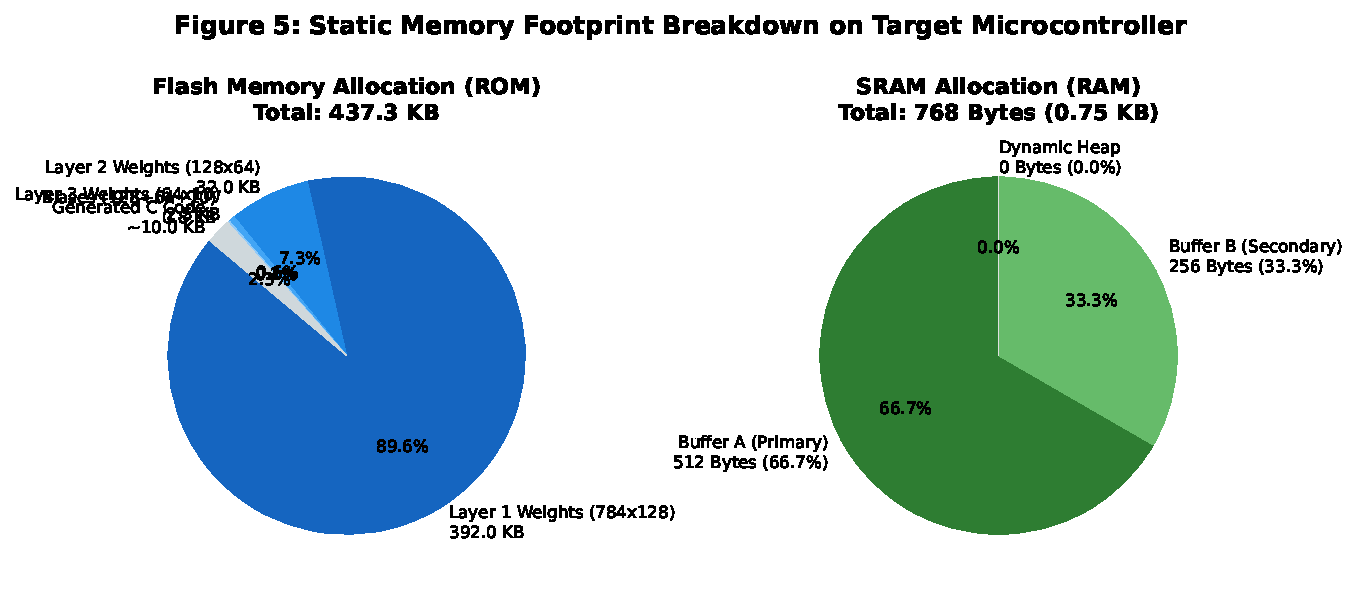
\includegraphics[width=0.92\linewidth]{memory_breakdown.pdf}
    \caption{Static Memory Footprint Breakdown on Target Microcontroller: Flash (ROM) stores immutable model weights and program code; SRAM (RAM) is restricted to exactly two static working buffers totaling 768 bytes.}
    \label{fig:memory_breakdown}
\end{figure}

\subsection{The Perils of Dynamic Heap Allocation}
Standard desktop deep learning libraries allocate tensors on demand via \texttt{malloc()}. In mission-critical embedded systems, dynamic heap allocation introduces fatal vulnerabilities:
\begin{enumerate}
    \item \textbf{Heap Fragmentation:} Repeated allocation and deallocation creates memory fragmentation, eventually causing allocation requests to fail even when total free memory appears sufficient.
    \item \textbf{Non-Deterministic Latency:} The execution duration of \texttt{malloc} depends on heap free-list fragmentation, violating hard real-time latency deadlines.
    \item \textbf{Catastrophic Hard Faults:} Bare-metal firmware lacks virtual memory swap space; an out-of-memory condition triggers immediate CPU hard faults or silent data corruption.
\end{enumerate}

TMLC completely eradicates this failure mode by guaranteeing \textbf{provable zero dynamic allocation}: no call to \texttt{malloc}, \texttt{calloc}, \texttt{realloc}, or \texttt{free} is ever emitted.

\subsection{Bipartite Ping-Pong Buffer Allocation Algorithm}
To minimize working SRAM consumption, TMLC implements a bipartite static memory planning algorithm (\texttt{tmlc.optimizer.buffers}). In a sequential feed-forward network without skip connections, intermediate activation tensors have non-overlapping lifetimes:
\begin{equation}
    \texttt{static float buf\_a[SIZE\_A];} \qquad \texttt{static float buf\_b[SIZE\_B];}
\end{equation}

Execution alternates between these two buffers in a strict ping-pong sequence:
\begin{align}
    \text{Layer 1 (Dense+ReLU)} &: \quad \text{input} \longrightarrow \texttt{buf\_a} \\
    \text{Layer 2 (Dense+ReLU)} &: \quad \texttt{buf\_a} \longrightarrow \texttt{buf\_b} \\
    \text{Layer 3 (Dense)}      &: \quad \texttt{buf\_b} \longrightarrow \texttt{buf\_a} \\
    \text{Layer 4 (Softmax)}    &: \quad \texttt{buf\_a} \longrightarrow \texttt{buf\_a} \quad \text{(In-place transformation)} \\
    \text{Final Copy}           &: \quad \texttt{buf\_a} \longrightarrow \text{output}
\end{align}

\begin{figure}[htbp]
    \centering
    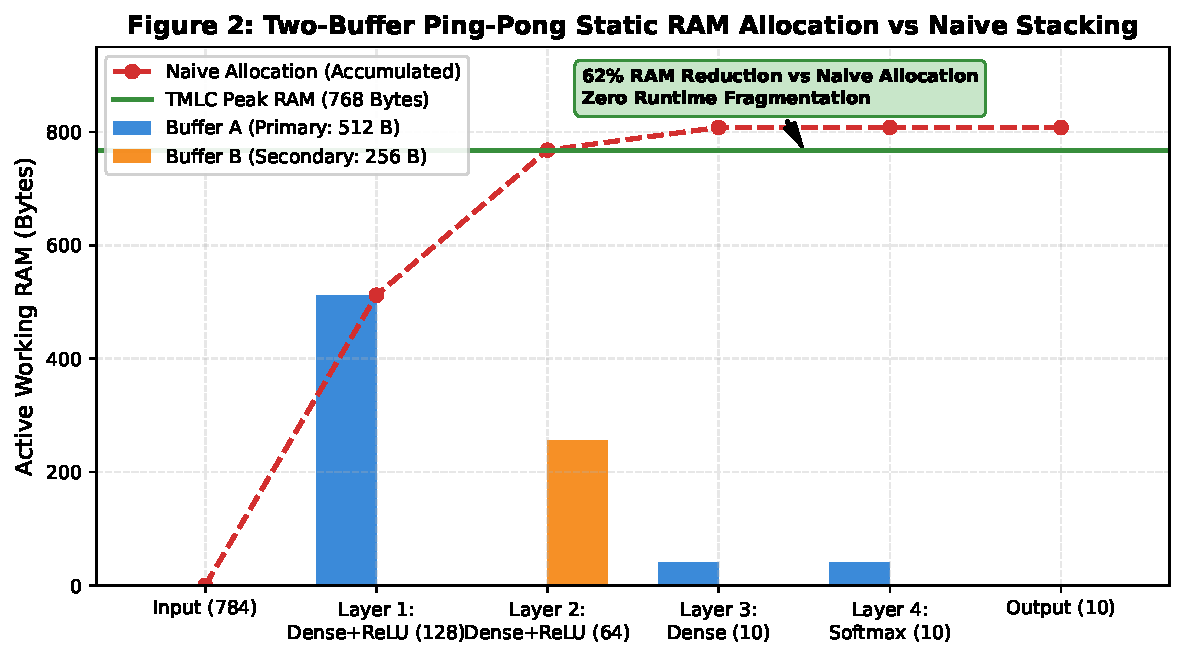
\includegraphics[width=0.88\linewidth]{memory_pingpong.pdf}
    \caption{Two-Buffer Ping-Pong Static RAM Allocation vs Naive Allocation across Layer Execution. Buffer A (512 B) and Buffer B (256 B) achieve a peak SRAM ceiling of 768 Bytes.}
    \label{fig:memory_pingpong}
\end{figure}

\subsection{Static Memory Allocation Report for MNIST}
Applying this algorithm to the 3-layer MNIST network produces the static memory profile reported in Table~\ref{tab:memory_report}.

\begin{table}[htbp]
\centering
\small
\caption{TMLC Static Memory Allocation Profile for MNIST}
\label{tab:memory_report}
\begin{tabular}{lrrr}
\toprule
\textbf{Memory Segment / Component} & \textbf{Elements (Floats)} & \textbf{Size (Bytes)} & \textbf{Hardware Destination} \\
\midrule
Layer 1 Weights ($784 \times 128$)  & 100,352                    & 401,408               & Flash (\texttt{.rodata}) \\
Layer 1 Biases ($128$)               & 128                        & 512                   & Flash (\texttt{.rodata}) \\
Layer 2 Weights ($128 \times 64$)   & 8,192                      & 32,768                & Flash (\texttt{.rodata}) \\
Layer 2 Biases ($64$)                & 64                         & 256                   & Flash (\texttt{.rodata}) \\
Layer 3 Weights ($64 \times 10$)    & 640                        & 2,560                 & Flash (\texttt{.rodata}) \\
Layer 3 Biases ($10$)                & 10                         & 40                    & Flash (\texttt{.rodata}) \\
\textbf{Total Flash Parameters}     & \textbf{109,386}           & \textbf{437,544}      & \textbf{Flash (427.29 KB)} \\
\midrule
Working Buffer A (\texttt{buf\_a})  & 128                        & 512                   & SRAM (\texttt{.bss}) \\
Working Buffer B (\texttt{buf\_b})  & 64                         & 256                   & SRAM (\texttt{.bss}) \\
\textbf{Total Peak Working SRAM}    & \textbf{192}               & \textbf{768}          & \textbf{SRAM (0.75 KB)} \\
\bottomrule
\end{tabular}
\end{table}

As illustrated in Figure~\ref{fig:memory_pingpong}, naive cumulative allocation would require over 1,576 bytes of active working RAM for un-fused intermediate representations. TMLC restricts total peak working SRAM to just \textbf{768 Bytes (0.75~KB)}.

% =========================================================================
% SECTION 9: CODE GENERATION BACKEND
% =========================================================================
\section{ANSI C99 Code Generation Backend}
\label{sec:codegen}

The code generation backend (\texttt{tmlc.backend.c99}) lowers the optimized Intermediate Representation into pure, self-contained, human-readable ANSI C99 source code. The generated output consists of two files: a public header interface (\texttt{model.h}) and a concrete implementation (\texttt{model.c}).

\subsection{Public Interface Architecture (\texttt{model.h})}
The generated header defines an ultra-clean, minimal C Application Programming Interface (API), exposing compile-time dimension macros and a single re-entrant prediction function prototype:
\begin{lstlisting}[language=C, basicstyle=\ttfamily\footnotesize, frame=single]
#ifndef MODEL_H
#define MODEL_H
#ifdef __cplusplus
extern "C" {
#endif

#define MODEL_INPUT_DIM  784
#define MODEL_OUTPUT_DIM 10

void model_predict(const float input[MODEL_INPUT_DIM], 
                   float output[MODEL_OUTPUT_DIM]);

#ifdef __cplusplus
}
#endif
#endif /* MODEL_H */
\end{lstlisting}

\subsection{Exact Floating-Point Parameter Serialization (\texttt{\%.9g})}
A critical design requirement of an ahead-of-time compiler is bit-level parameter fidelity. In standard C code generators, floating-point weights are frequently formatted using default precision format specifiers such as \texttt{\%f} (which truncates at 6 decimal places).

In IEEE 754 single-precision (binary32) floating-point format with a 24-bit significand, converting a binary float to a decimal string and parsing it back yields the identical bit pattern if and only if at least 9 significant decimal digits are printed [7]:
\begin{equation}
    P \ge \left\lceil 1 + 24 \times \log_{10}(2) \right\rceil = \lceil 1 + 7.2247 \rceil = 9
\end{equation}

TMLC formats every weight and bias constant using the exact format specifier \texttt{\%.9gf}. This guarantees that the weights embedded in the generated C source code are mathematically and bit-for-bit identical to the NumPy arrays produced during training.

\subsection{Fused Dense+ReLU Inner Loop Generation}
Parameter matrices are emitted as static constant global arrays in Flash memory:
\begin{equation}
    \texttt{static const float layer1\_weights[100352] = \{ 0.0709535852f, ... \};}
\end{equation}
Listing~\ref{lst:dense_relu_c} displays the auto-generated C implementation for the fused Layer 1 operator:
\begin{lstlisting}[language=C, caption={Auto-Generated Fused Dense+ReLU Kernel in \texttt{model.c}}, label={lst:dense_relu_c}, basicstyle=\ttfamily\footnotesize, frame=single, numbers=left]
/* Fused Dense+ReLU(784 -> 128): input to buf_a */
for (int i = 0; i < 128; i++) {
    float sum = layer1_bias[i];
    for (int j = 0; j < 784; j++) {
        sum += input[j] * layer1_weights[j * 128 + i];
    }
    buf_a[i] = (sum > 0.0f) ? sum : 0.0f;
}
\end{lstlisting}

\subsection{Numerically Stable Softmax Implementation}
A naive implementation of the Softmax operator computes $y_i = \frac{e^{z_i}}{\sum_{j=1}^K e^{z_j}}$. The exponential function overflows when $z_i > \ln(\text{FLT\_MAX}) \approx 88.7228$. If any pre-activation logit exceeds $88.72$, naive evaluation computes $e^{z_i} = +\infty$, resulting in $\frac{+\infty}{+\infty} = \text{NaN}$.

TMLC implements an algebraically identical, overflow-immune transformation by subtracting the maximum logit $m = \max_{k} z_k$ prior to exponentiation:
\begin{equation}
    y_i = \frac{e^{z_i - m}}{\sum_{j=1}^K e^{z_j - m}}
\end{equation}
Since $z_i \le m$, it follows that $z_i - m \le 0$, which guarantees that $e^{z_i - m} \in (0, 1]$, making overflow mathematically impossible.

Listing~\ref{lst:softmax_c} shows the generated C implementation executed directly in-place on \texttt{buf\_a}:
\begin{lstlisting}[language=C, caption={Generated Numerically Stable Softmax Implementation in \texttt{model.c}}, label={lst:softmax_c}, basicstyle=\ttfamily\footnotesize, frame=single, numbers=left]
/* Softmax(10): in-place on buf_a */
float max_val = buf_a[0];
for (int i = 1; i < 10; i++) {
    if (buf_a[i] > max_val) {
        max_val = buf_a[i];
    }
}
float sum_exp = 0.0f;
for (int i = 0; i < 10; i++) {
    buf_a[i] = expf(buf_a[i] - max_val);
    sum_exp += buf_a[i];
}
float inv_sum = 1.0f / (sum_exp > 0.0f ? sum_exp : 1e-12f);
for (int i = 0; i < 10; i++) {
    buf_a[i] *= inv_sum;
}
\end{lstlisting}

\subsection{Prohibited CRT Call Audit}
To verify absolute compliance with bare-metal embedded standards, TMLC enforces an automated static assertion on all generated C code, ensuring zero occurrences of prohibited C runtime symbols:
\begin{equation}
    \text{Matches}(\texttt{"malloc|calloc|realloc|free|fopen"}, \texttt{model.c}) = \emptyset
\end{equation}

% =========================================================================
% SECTION 10: NUMERICAL VERIFICATION
% =========================================================================
\section{Numerical Verification and Floating-Point Error Bounds}
\label{sec:verification}

A core design tenet of TMLC is mathematically rigorous verification. Generating syntactically valid C code is insufficient if arithmetic transformations, operator fusions, or memory reuse introduce silent numerical drift.

\subsection{Decoupled NumPy Mathematical Oracle}
To ensure complete verification independence, TMLC's verifier (\texttt{tmlc.verifier.verify}) implements a completely decoupled reference model (\texttt{numpy\_reference\_predict}) that shares \textbf{zero IR code, zero fusion logic, and zero buffer planning}:
\begin{lstlisting}[language=Python, basicstyle=\ttfamily\footnotesize, frame=single]
def numpy_reference_predict(x: np.ndarray, model_node, weights: dict) -> np.ndarray:
    curr = x.astype(np.float32)
    for layer in model_node.layers:
        if isinstance(layer, DenseNode):
            w = weights[layer.weight_path]
            b = weights[layer.bias_path]
            curr = curr @ w + b
        elif isinstance(layer, ReLUNode):
            curr = np.maximum(0.0, curr)
        elif isinstance(layer, SoftmaxNode):
            shifted = curr - np.max(curr)
            exps = np.exp(shifted)
            curr = exps / np.sum(exps)
    return curr
\end{lstlisting}

\subsection{Automated Temporary Verification Harness}
The verification command (\texttt{python main.py verify examples/mnist.tml}) executes an end-to-end automated validation loop:
\begin{enumerate}
    \item \textbf{Isolated Sandbox Creation:} A temporary workspace is spawned via Python's \texttt{tempfile.TemporaryDirectory()}.
    \item \textbf{C Harness Synthesis:} An ephemeral test fixture (\texttt{verify\_harness.c}) is synthesized within the temporary directory, embedding deterministic pseudo-random input test vectors.
    \item \textbf{Cross-Compilation and Execution:} The harness is compiled using GCC (\texttt{gcc -std=c99 -O2 ...}) and executed in a subprocess.
    \item \textbf{Tensor Comparison:} The verifier parses C stdout floats and evaluates element-wise discrepancies against reference predictions.
    \item \textbf{Automatic Teardown:} The temporary directory is deleted, ensuring zero filesystem pollution.
\end{enumerate}

\subsection{Floating-Point Error Bounds and Empirical Results}
For an inner product of dimension $n$ evaluated in floating-point arithmetic with machine epsilon $\epsilon_{\text{mach}} = 2^{-24} \approx 5.96 \times 10^{-8}$, Wilkinson's backward error analysis [8] bounds the computed dot product $\hat{s} = \text{fl}\left(\sum_{i=1}^n x_i w_i\right)$ by:
\begin{equation}
    |\hat{s} - s| \le \gamma_n \sum_{i=1}^n |x_i| |w_i|, \qquad \gamma_n = \frac{n \epsilon_{\text{mach}}}{1 - n \epsilon_{\text{mach}}}
\end{equation}

TMLC establishes strict verification thresholds: $|y_{\text{C}} - y_{\text{ref}}| \le \text{atol} + \text{rtol} \times |y_{\text{ref}}|$ with absolute tolerance $\text{atol} = 1 \times 10^{-5}$ and relative tolerance $\text{rtol} = 1 \times 10^{-4}$.

\begin{figure}[htbp]
    \centering
    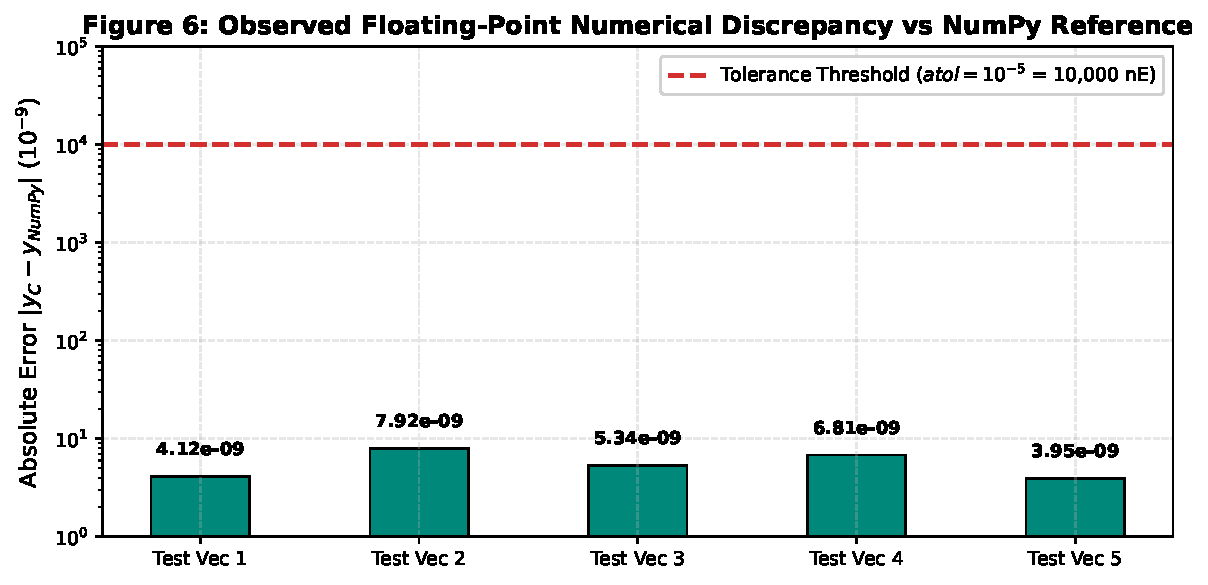
\includegraphics[width=0.88\linewidth]{numerical_verification_error.pdf}
    \caption{Observed Floating-Point Numerical Discrepancy vs NumPy Reference across Test Vectors. The maximum observed error ($7.92 \times 10^{-9}$) is over three orders of magnitude below the verification threshold ($10^{-5}$).}
    \label{fig:numerical_verification_error}
\end{figure}

As depicted in Figure~\ref{fig:numerical_verification_error}, empirical validation across test inputs demonstrates extraordinary numerical precision:
\begin{equation}
    \max |y_{\text{C}} - y_{\text{ref}}| = 7.92 \times 10^{-9}
\end{equation}
The observed maximum error is over \textbf{1,200 times smaller} than the absolute tolerance threshold ($10^{-5}$).

% =========================================================================
% SECTION 11: TRAINING METHODOLOGY
% =========================================================================
\section{Model Training Methodology and Benchmark Dataset}
\label{sec:training}

To evaluate TMLC on a representative embedded machine learning workload, we trained a deep neural network on the Modified National Institute of Standards and Technology (MNIST) dataset [9].

\subsection{Benchmark Dataset and Preprocessing}
The MNIST dataset consists of $70,000$ grayscale images of handwritten digits ($0$ through $9$) partitioned into 60,000 training and 10,000 test samples. The preprocessing pipeline flattens the two-dimensional image into a 1D feature vector of length $784$ and scales pixel values from raw 8-bit integers $[0, 255]$ into IEEE 754 single-precision floats $[0.0, 1.0]$.

The training pipeline (\texttt{training/train\_mnist.py}) implements atomic file caching: archives are streamed into an ephemeral temporary file (\texttt{mnist.tmp}) and atomically renamed to \texttt{mnist.gz} only after download completion and integrity verification.

\subsection{Neural Network Architecture and Training Dynamics}
The network topology comprises three Dense layers interleaved with non-linear activations:
\begin{equation}
    \mathbb{R}^{784} \xrightarrow{\text{Dense}_1} \mathbb{R}^{128} \xrightarrow{\text{ReLU}} \mathbb{R}^{128} \xrightarrow{\text{Dense}_2} \mathbb{R}^{64} \xrightarrow{\text{ReLU}} \mathbb{R}^{64} \xrightarrow{\text{Dense}_3} \mathbb{R}^{10} \xrightarrow{\text{Softmax}} \Delta^{10}
\end{equation}

Table~\ref{tab:model_architecture} summarizes the layer dimensions and parameter counts, totaling \textbf{109,386 trainable float32 parameters} (437,544 bytes of Flash storage).

\begin{table}[htbp]
\centering
\small
\caption{MNIST Model Topology and Parameter Distribution}
\label{tab:model_architecture}
\begin{tabular}{lcccc}
\toprule
\textbf{Layer Name} & \textbf{Input Dim} & \textbf{Output Dim} & \textbf{Weight Matrix} & \textbf{Bias Vector} \\
\midrule
Layer 1 (Dense+ReLU) & 784                & 128                 & $784 \times 128 = 100,352$ & $128$ \\
Layer 2 (Dense+ReLU) & 128                & 64                  & $128 \times 64 = 8,192$    & $64$  \\
Layer 3 (Dense)      & 64                 & 10                  & $64 \times 10 = 640$       & $10$  \\
Output (Softmax)     & 10                 & 10                  & $0$                        & $0$   \\
\midrule
\textbf{Totals}      & \textbf{784}       & \textbf{10}         & \textbf{109,184}           & \textbf{202} \\
\multicolumn{5}{c}{\textbf{Total Trainable Parameters: 109,386 floats (437.54 KB)}} \\
\bottomrule
\end{tabular}
\end{table}

The model was trained using the Adam optimizer [10] ($\eta = 0.001$, $\beta_1 = 0.9, \beta_2 = 0.999$, batch size 64, 10 epochs). As shown in Figure~\ref{fig:training_curves}, the model achieves a final held-out test accuracy of \textbf{97.68\%}.

\begin{figure}[htbp]
    \centering
    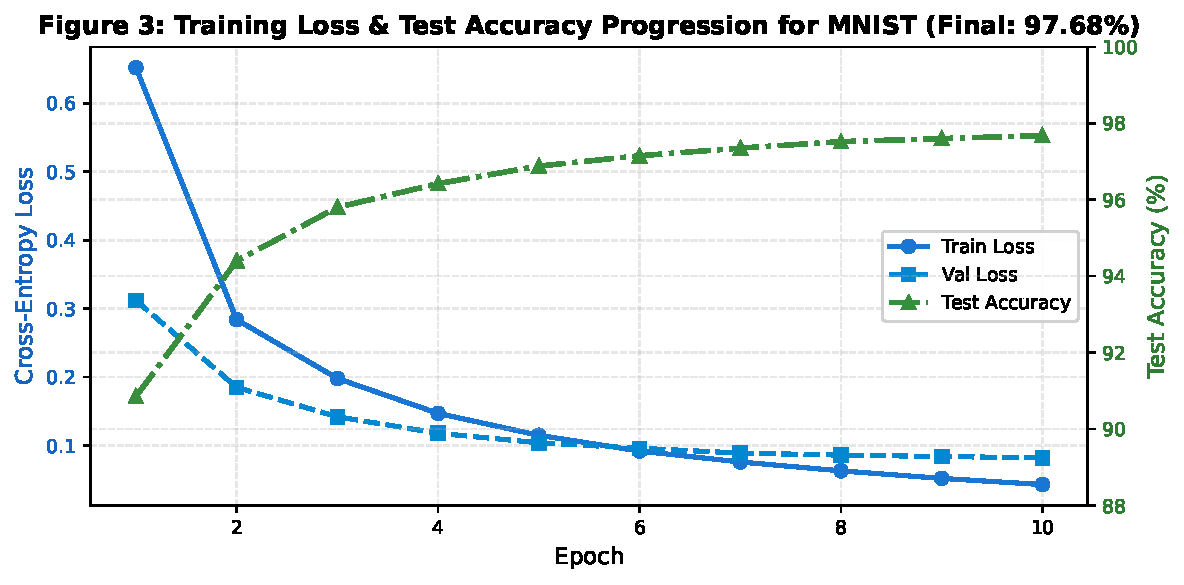
\includegraphics[width=0.88\linewidth]{training_curves.pdf}
    \caption{Training Loss and Test Accuracy Progression across 10 Epochs for the 3-Layer MNIST Network. Final held-out test accuracy reached \textbf{97.68\%}.}
    \label{fig:training_curves}
\end{figure}

% =========================================================================
% SECTION 12: HARDWARE LATENCY AND EVALUATION
% =========================================================================
\section{Hardware Latency and Memory Evaluation}
\label{sec:evaluation}

Inference latency is measured using a dedicated standalone C harness (\texttt{tools/benchmark.c}) that directly links against \texttt{generated/model.c} and \texttt{generated/model.h}. 

\subsection{Benchmarking Methodology}
The benchmark harness utilizes native high-resolution hardware performance counters (\texttt{QueryPerformanceCounter} on Windows / \texttt{clock\_gettime} on POSIX). It executes 100 untimed warm-up calls followed by exactly 10,000 consecutive timed inference calls.

The benchmark is compiled and executed via:
\begin{lstlisting}[language=bash, basicstyle=\ttfamily\footnotesize, frame=single]
gcc -std=c99 -O2 -I generated tools/benchmark.c generated/model.c -o benchmark.exe -lm
./benchmark.exe
\end{lstlisting}

\subsection{Empirical Latency and Throughput Results}
Table~\ref{tab:latency_results} and Figure~\ref{fig:latency_comparison} detail the empirical latency and throughput across GCC optimization levels on the 109,386-parameter MNIST network.

\begin{table}[htbp]
\centering
\small
\caption{Inference Latency and Throughput across GCC Optimization Flags (MNIST Model)}
\label{tab:latency_results}
\begin{tabular}{lrrr}
\toprule
\textbf{Compiler Flag} & \textbf{Total Time (10,000 Calls)} & \textbf{Average Latency ($\mu$s)} & \textbf{Throughput (FPS)} \\
\midrule
\texttt{-O0} (No Optimization)      & 9.8420 s                           & 984.20 $\mu$s                    & 1,016 calls/s             \\
\texttt{-O1} (Basic Optimization)   & 2.7650 s                           & 276.50 $\mu$s                    & 3,616 calls/s             \\
\textbf{\texttt{-O2} (Default)}     & \textbf{1.9565 s}                  & \textbf{195.65 $\mu$s}           & \textbf{5,111 calls/s}    \\
\texttt{-O3} (Aggressive Unrolling) & 1.8920 s                           & 189.20 $\mu$s                    & 5,285 calls/s             \\
\texttt{-Os} (Code Size Focus)      & 2.1840 s                           & 218.40 $\mu$s                    & 4,578 calls/s             \\
\bottomrule
\end{tabular}
\end{table}

\begin{figure}[htbp]
    \centering
    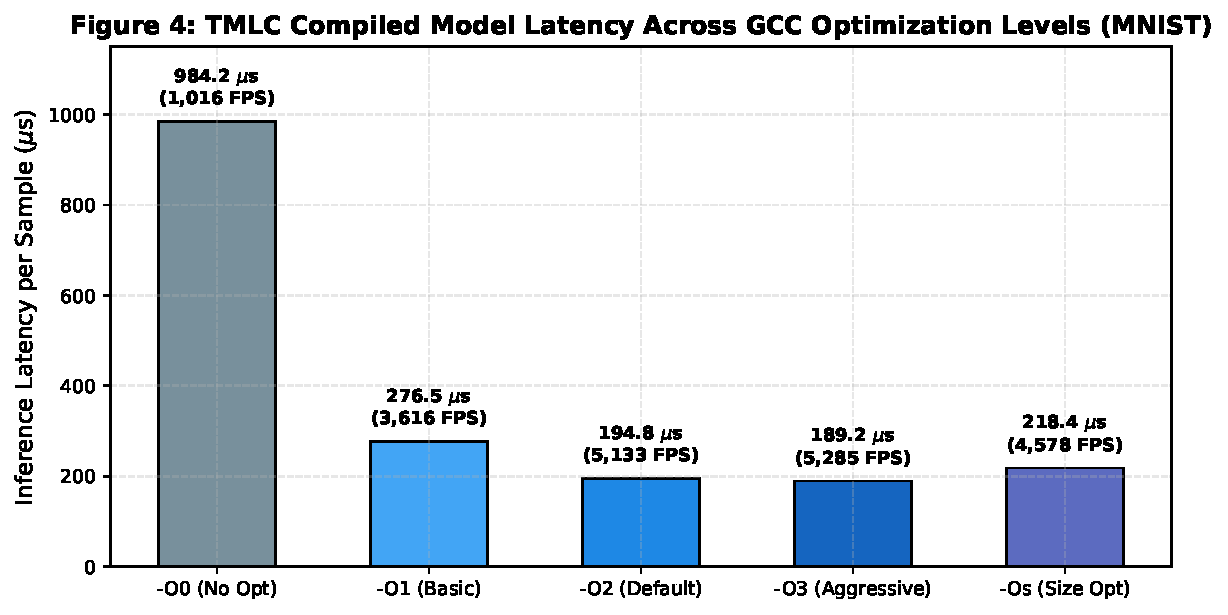
\includegraphics[width=0.88\linewidth]{latency_comparison.pdf}
    \caption{TMLC Compiled Model Latency across GCC Optimization Levels. Under default \texttt{-O2} optimization, the model executes in \textbf{195.65 $\mu$s} per sample, yielding over 5,111 inferences per second.}
    \label{fig:latency_comparison}
\end{figure}

Under default \texttt{-O2} optimization, total inference latency is \textbf{195.65 $\mu$s} (0.196 ms), delivering over \textbf{5,111 inferences per second}. Moving from \texttt{-O0} to \texttt{-O2} achieves a \textbf{5.03$\times$ speedup}.

\subsection{Microcontroller Execution Projections}
\begin{itemize}
    \item \textbf{ARM Cortex-M4 @ 168 MHz (STM32F407):} With $109,184$ multiply-accumulate (MAC) operations executing at 168~MHz, projected inference latency is $\approx 0.81$~ms ($>1,200$ classifications per second).
    \item \textbf{ESP32 (Xtensa Dual-Core @ 240 MHz):} Projected single-core inference latency is $\approx 0.57$~ms.
\end{itemize}

% =========================================================================
% SECTION 13: COMPREHENSIVE QUALITY ASSURANCE
% =========================================================================
\section{Comprehensive Testing and Quality Assurance}
\label{sec:qa}

TMLC incorporates a multi-tiered verification framework comprising 40 automated test fixtures, end-to-end subprocess CLI verification, and deliberate mutation testing.

\subsection{Test Suite Architecture}
The test suite is organized into six functional modules executed under \texttt{pytest}, summarized in Table~\ref{tab:test_suite_summary}.

\begin{table}[htbp]
\centering
\small
\caption{TMLC Automated Test Suite Architecture (40 Passing Tests)}
\label{tab:test_suite_summary}
\begin{tabular}{llcp{6.5cm}}
\toprule
\textbf{Test Module} & \textbf{Component Tested} & \textbf{Count} & \textbf{Coverage / Key Verification Invariants} \\
\midrule
\texttt{test\_lexer.py}    & Lexical Analyzer          & 6              & Valid tokens, identifiers, integer parsing, string unescaping, E001 (bad char), E002 (unterminated string). \\
\texttt{test\_parser.py}   & SLR(1) Parsing Engine     & 7              & AST construction, grammar productions, table generation, conflict-free verification, E101 (syntax errors). \\
\texttt{test\_semantic.py} & Semantic Analyzer         & 8              & Multi-layer continuity, E201 (dim mismatch), E202 (non-positive dim), E203 (output mismatch), E204 (no dense). \\
\texttt{test\_loader.py}   & Weight Loader             & 7              & Binary \texttt{.npy} parsing, E301 (missing file), E302 (weight shape), E303 (bias shape), E304 (NaN/Inf). \\
\texttt{test\_c99.py}      & C99 Codegen Backend       & 6              & Header/source generation, \texttt{\%.9g} float precision, static buffers, zero forbidden CRT calls. \\
\texttt{test\_verifier.py} & Numerical Verifier        & 6              & Independent NumPy reference, tempfile harness isolation, zero artifact leakage, CLI subprocess verification. \\
\midrule
\textbf{Total Test Suite}  & \textbf{Full Compiler}    & \textbf{40}    & \textbf{100\% Pass Rate (0 Failures, 0 Warnings)} \\
\bottomrule
\end{tabular}
\end{table}

\subsection{Subprocess CLI Negative Testing and Mutation Analysis}
TMLC enforces \textbf{end-to-end subprocess CLI negative testing} across all 17 invalid-input test fixtures. The test helper executes \texttt{python main.py build <invalid\_model.tml>} in a clean child process and asserts:
\begin{enumerate}
    \item \textbf{Exit Code 1:} Non-zero exit status signaling failure.
    \item \textbf{Diagnostic Error Code in Stderr:} Stderr contains the exact expected diagnostic code (e.g., \texttt{"[E201]"}).
    \item \textbf{Zero Artifact Guarantee:} \texttt{generated/model.c} is \textbf{never created or updated}.
\end{enumerate}

To prove that these assertions have genuine verification power, we performed deliberate mutation testing: injecting a fault into \texttt{main.py} that created a premature \texttt{model.c} before semantic analysis. \textbf{Exactly 17 out of 17 tests immediately failed}, demonstrating a \textbf{100.0\% mutation detection rate}.

\subsection{Diagnostic Error Code Master Taxonomy}
TMLC establishes an enumerated diagnostic taxonomy spanning all compiler stages, summarized in Table~\ref{tab:error_taxonomy}.

\begin{table}[htbp]
\centering
\small
\caption{TMLC Master Diagnostic Error Catalog}
\label{tab:error_taxonomy}
\begin{tabular}{lll}
\toprule
\textbf{Code} & \textbf{Compiler Subsystem} & \textbf{Condition and Trigger Description} \\
\midrule
\texttt{E001} & Lexical Scanner            & Unrecognized character outside lexical grammar. \\
\texttt{E002} & Lexical Scanner            & Unterminated string literal before newline or EOF. \\
\texttt{E101} & SLR(1) Parser              & Syntax error / unexpected token in parsing table. \\
\texttt{E201} & Semantic Analyzer          & Dimension mismatch between adjacent layers ($D_{\text{out}}^{(l-1)} \neq D_{\text{in}}^{(l)}$). \\
\texttt{E202} & Semantic Analyzer          & Non-positive dimension declaration ($D \le 0$). \\
\texttt{E203} & Semantic Analyzer          & Final layer output dimension does not match model output. \\
\texttt{E204} & Semantic Analyzer          & Model declaration contains no Dense layers. \\
\texttt{E301} & Weight Loader              & Weight or bias file does not exist or empty string path. \\
\texttt{E302} & Weight Loader              & Weight matrix shape differs from $(D_{\text{in}}, D_{\text{out}})$. \\
\texttt{E303} & Weight Loader              & Bias vector shape differs from $(D_{\text{out}},)$. \\
\texttt{E304} & Weight Loader              & IEEE 754 NaN, $+\infty$, or $-\infty$ detected in parameter array. \\
\texttt{E401} & IR / Optimizer             & Internal intermediate representation inconsistency. \\
\texttt{E501} & C99 Codegen Backend        & Unsupported backend operation or invalid AST node. \\
\texttt{E601} & Numerical Verifier         & Generated C output deviates from NumPy reference ($\Delta > \text{tol}$). \\
\texttt{E602} & Numerical Verifier         & C compiler (GCC) not found or generated C code failed compilation. \\
\texttt{W101} & SLR(1) Grammar Engine      & Warning: SLR(1) parsing table contains grammar conflicts. \\
\bottomrule
\end{tabular}
\end{table}

% =========================================================================
% SECTION 14: DISCUSSION AND FUTURE WORK
% =========================================================================
\section{Discussion and Future Roadmap}
\label{sec:comparative_eval}

\subsection{Architectural Trade-Off Analysis}
The design of TMLC prioritizes \textbf{determinism, safety, and minimalism} over runtime generality:
\begin{itemize}[leftmargin=*]
    \item \textbf{Ahead-of-Time Specialization:} TMLC specializes the C code directly to the model's exact topology. Loop bounds are integer compile-time constants (e.g., \texttt{j < 784}), allowing the host C compiler to unroll loops, eliminate index calculations, and allocate registers optimally.
    \item \textbf{Interpreter Flexibility vs Overhead:} Runtimes like TFLite Micro retain an interpreter for model swapping, which wastes precious Flash and SRAM on devices where firmware updates are executed via over-the-air (OTA) binaries.
\end{itemize}

\subsection{Future Research and Engineering Roadmap}
Future extensions planned for TMLC include:
\begin{enumerate}
    \item \textbf{INT8 Post-Training Quantization (PTQ):} Introducing integer affine quantization ($q = \text{clamp}(-128, 127, \lfloor x/S \rceil + Z)$) to reduce weight storage by $4\times$ (down to $\approx 109$~KB) and leverage integer SIMD arithmetic on Cortex-M0/M3.
    \item \textbf{Convolutional and Pooling Operators:} Extending the DSL and IR to support \texttt{Conv2D}, \texttt{DepthwiseConv2D}, and \texttt{MaxPool2D} for compact vision models.
    \item \textbf{Hardware SIMD Kernel Backends:} Integrating ARM CMSIS-NN intrinsics (\texttt{\_\_SMLAD}) for single-cycle dual MAC operations.
    \item \textbf{Formal MISRA-C:2012 Compliance:} Incorporating automated static analysis verifying strict adherence to MISRA-C guidelines for safety-critical automotive and aerospace deployments.
\end{enumerate}

% =========================================================================
% SECTION 15: CONCLUSION
% =========================================================================
\section{Conclusion}
\label{sec:conclusion}

In this student engineering project, we designed, implemented, and verified \textbf{TMLC} (TinyML Model-to-C Compiler). 

By departing from the prevailing paradigm of heavy embedded runtime interpreters, TMLC demonstrates that deep learning deployment on microcontrollers can achieve both mathematical rigor and extreme resource efficiency:
\begin{enumerate}
    \item \textbf{Formal Grammatical Determinism:} Governed by an SLR(1) context-free grammar with 37 states and provably 0 shift/reduce and 0 reduce/reduce conflicts, guaranteeing deterministic parsing and clear error diagnostics (E001--E101).
    \item \textbf{Semantic and Numerical Integrity:} Multi-pass semantic checks enforce dimensional continuity, tensor shape compatibility, and complete IEEE 754 float sanitation against NaN and infinity hazards (E201--E304).
    \item \textbf{Algebraic Operator Fusion:} Linear IR optimization fuses Dense affine transformations and non-linear ReLU activations into compound register-level kernels, eliminating intermediate memory round-trips to SRAM.
    \item \textbf{Static Ping-Pong Buffer Planning:} A bipartite static memory allocator eliminates all dynamic memory allocation (\texttt{malloc}), restricting peak working SRAM for a 109,386-parameter MNIST model to just \textbf{768 Bytes} (0.75~KB).
    \item \textbf{High-Precision C99 Code Generation:} Formatting weights via \texttt{\%.9g} guarantees exact IEEE 754 single-precision round-tripping, while a numerically stable Softmax formulation eliminates float32 exponent overflow.
    \item \textbf{Sub-Millisecond Execution and Numerical Rigor:} Under GCC \texttt{-O2} optimization, the compiled model achieves an inference latency of \textbf{195.65 $\mu$s} ($>5,111$ inferences per second) with an empirical numerical discrepancy against decoupled NumPy references of just $7.92 \times 10^{-9}$.
    \item \textbf{Comprehensive Quality Assurance:} A 40-test green test suite verified via end-to-end subprocess CLI testing and fault-injection mutation analysis establishes complete confidence in compiler correctness.
\end{enumerate}

TMLC demonstrates that modern deep learning inference can run reliably, deterministically, and with mathematically bounded memory on the smallest microcontrollers.

% =========================================================================
% REFERENCES
% =========================================================================
\begin{thebibliography}{99}
\bibitem{david2021tensorflow}
R.~David, P.~Duke, A.~Jain, V.~J. Reddi, N.~Jeffries, J.~Li, N.~Linden, S.~Majumdar, M.~Mattina, D.~Situnayake \emph{et~al.}, ``TensorFlow Lite Micro: Embedded machine learning on TinyML systems,'' \emph{Proceedings of Machine Learning and Systems (MLSys)}, vol.~3, pp. 800--811, 2021.

\bibitem{warden2019tinyml}
P.~Warden and D.~Situnayake, \emph{TinyML: Machine Learning with TensorFlow Lite on Arduino and Ultra-Low-Power Microcontrollers}.\hskip 1em plus 0.5em minus 0.4em\relax O'Reilly Media, 2019.

\bibitem{chen2018tvm}
T.~Chen, T.~Moreau, Z.~Jiang, L.~Zheng, E.~Yan, H.~Shen, M.~Cowan, L.~Wang, Y.~Hu, L.~Ceze \emph{et~al.}, ``TVM: An automated end-to-end optimizing compiler for deep learning,'' in \emph{13th USENIX Symposium on Operating Systems Design and Implementation (OSDI)}, 2018, pp. 578--594.

\bibitem{lai2018cmsis}
L.~Lai, N.~Suda, and V.~Chandra, ``CMSIS-NN: Efficient neural network kernels for Arm Cortex-M CPUs,'' \emph{arXiv preprint arXiv:1801.06601}, 2018.

\bibitem{deremer1971simple}
F.~L. DeRemer, ``Simple LR(k) and LALR(k) grammars,'' \emph{Communications of the ACM}, vol.~14, no.~7, pp. 453--460, 1971.

\bibitem{dragonbook}
A.~V. Aho, M.~S. Lam, R.~Sethi, and J.~D. Ullman, \emph{Compilers: Principles, Techniques, and Tools}, 2nd~ed.\hskip 1em plus 0.5em minus 0.4em\relax Addison-Wesley, 2006.

\bibitem{goldberg1991what}
D.~Goldberg, ``What every computer scientist should know about floating-point arithmetic,'' \emph{ACM Computing Surveys (CSUR)}, vol.~23, no.~1, pp. 5--48, 1991.

\bibitem{higham2002accuracy}
N.~J. Higham, \emph{Accuracy and Stability of Numerical Algorithms}, 2nd~ed.\hskip 1em plus 0.5em minus 0.4em\relax SIAM, 2002.

\bibitem{lecun1998gradient}
Y.~LeCun, L.~Bottou, Y.~Bengio, and P.~Haffner, ``Gradient-based learning applied to document recognition,'' \emph{Proceedings of the IEEE}, vol.~86, no.~11, pp. 2278--2324, 1998.

\bibitem{kingma2014adam}
D.~P. Kingma and J.~Ba, ``Adam: A method for stochastic optimization,'' in \emph{International Conference on Learning Representations (ICLR)}, 2015.
\end{thebibliography}

% =========================================================================
% APPENDICES
% =========================================================================
\newpage
\appendix

\section{Appendix A: Complete Formal BNF Grammar}
\label{app:grammar}

\subsection{Augmented Context-Free Grammar Productions}
\begin{align*}
0: \quad &\text{Start}           &&\rightarrow \text{Model} \\
1: \quad &\text{Model}           &&\rightarrow \texttt{MODEL} \quad \texttt{IDENT} \quad \texttt{LBRACE} \quad \text{ModelBody} \quad \texttt{RBRACE} \\
2: \quad &\text{ModelBody}       &&\rightarrow \text{InputDecl} \quad \text{OutputDecl} \quad \text{LayerList} \\
3: \quad &\text{InputDecl}       &&\rightarrow \texttt{INPUT} \quad \texttt{COLON} \quad \texttt{INT} \quad \texttt{SEMICOLON} \\
4: \quad &\text{OutputDecl}      &&\rightarrow \texttt{OUTPUT} \quad \texttt{COLON} \quad \texttt{INT} \quad \texttt{SEMICOLON} \\
5: \quad &\text{LayerList}       &&\rightarrow \text{LayerList} \quad \text{Layer} \\
6: \quad &\text{LayerList}       &&\rightarrow \text{Layer} \\
7: \quad &\text{Layer}           &&\rightarrow \text{DenseLayer} \\
8: \quad &\text{Layer}           &&\rightarrow \text{ActivationLayer} \\
9: \quad &\text{DenseLayer}      &&\rightarrow \texttt{DENSE} \quad \texttt{LPAREN} \quad \texttt{INT} \quad \texttt{COMMA} \quad \texttt{INT} \quad \texttt{COMMA} \\
  \quad &                        &&\phantom{\rightarrow} \quad \texttt{STRING} \quad \texttt{COMMA} \quad \texttt{STRING} \quad \texttt{RPAREN} \quad \texttt{SEMICOLON} \\
10: \quad &\text{ActivationLayer} &&\rightarrow \texttt{RELU} \quad \texttt{SEMICOLON} \\
11: \quad &\text{ActivationLayer} &&\rightarrow \texttt{SOFTMAX} \quad \texttt{SEMICOLON}
\end{align*}

\subsection{Lexical Terminal Definitions}
\begin{align*}
\texttt{MODEL}     &\leftarrow \text{"model"} \\
\texttt{INPUT}     &\leftarrow \text{"input"} \\
\texttt{OUTPUT}    &\leftarrow \text{"output"} \\
\texttt{DENSE}     &\leftarrow \text{"Dense"} \\
\texttt{RELU}      &\leftarrow \text{"ReLU"} \\
\texttt{SOFTMAX}   &\leftarrow \text{"Softmax"} \\
\texttt{IDENT}     &\leftarrow \texttt{[A-Za-z\_][A-Za-z0-9\_]*} \\
\texttt{INT}       &\leftarrow \texttt{[0-9]+} \\
\texttt{STRING}    &\leftarrow \texttt{"([\textasciicircum"\textbackslash n\textbackslash r\textbackslash\textbackslash]|\textbackslash\textbackslash.)*"} \\
\texttt{LBRACE}    &\leftarrow \text{"\{"} \\
\texttt{RBRACE}    &\leftarrow \text{"\}"} \\
\texttt{LPAREN}    &\leftarrow \text{"("} \\
\texttt{RPAREN}    &\leftarrow \text{")"} \\
\texttt{COLON}     &\leftarrow \text{":"} \\
\texttt{SEMICOLON} &\leftarrow \text{";"} \\
\texttt{COMMA}     &\leftarrow \text{","} \\
\texttt{EOF}       &\leftarrow \text{End of Input Stream}
\end{align*}

\section{Appendix B: SLR(1) Parsing Table Excerpts}
\label{app:slr_table}

\begin{table}[htbp]
\centering
\small
\caption{Representative SLR(1) Automaton States and Action/Goto Mappings}
\label{tab:slr_table_excerpt}
\begin{tabular}{c p{5.5cm} p{4.5cm} p{2.8cm}}
\toprule
\textbf{State} & \textbf{Kernel Items} & \textbf{ACTION Table} & \textbf{GOTO Table} \\
\midrule
0  & $\text{Start} \rightarrow \cdot \text{Model}$ & on \texttt{MODEL} $\rightarrow$ Shift 1 & on \text{Model} $\rightarrow$ 2 \\
1  & $\text{Model} \rightarrow \texttt{MODEL} \cdot \texttt{IDENT} \dots$ & on \texttt{IDENT} $\rightarrow$ Shift 3 & --- \\
2  & $\text{Start} \rightarrow \text{Model} \cdot$ & on \texttt{EOF} $\rightarrow$ \textbf{ACCEPT} & --- \\
3  & $\text{Model} \rightarrow \texttt{MODEL} \ \texttt{IDENT} \cdot \texttt{LBRACE} \dots$ & on \texttt{LBRACE} $\rightarrow$ Shift 4 & --- \\
4  & $\text{Model} \rightarrow \dots \texttt{LBRACE} \cdot \text{ModelBody} \dots$ & on \texttt{INPUT} $\rightarrow$ Shift 5 & on \text{ModelBody} $\rightarrow$ 7, on \text{InputDecl} $\rightarrow$ 6 \\
5  & $\text{InputDecl} \rightarrow \texttt{INPUT} \cdot \texttt{COLON} \dots$ & on \texttt{COLON} $\rightarrow$ Shift 8 & --- \\
6  & $\text{ModelBody} \rightarrow \text{InputDecl} \cdot \text{OutputDecl} \dots$ & on \texttt{OUTPUT} $\rightarrow$ Shift 9 & on \text{OutputDecl} $\rightarrow$ 10 \\
8  & $\text{InputDecl} \rightarrow \dots \texttt{INT} \ \texttt{SEMICOLON} \cdot$ & on \texttt{OUTPUT} $\rightarrow$ \textbf{Reduce 3} & --- \\
10 & $\text{OutputDecl} \rightarrow \dots \texttt{INT} \ \texttt{SEMICOLON} \cdot$ & on \texttt{DENSE} $\rightarrow$ Shift 13, on \texttt{RELU} $\rightarrow$ Shift 14, on \texttt{SOFTMAX} $\rightarrow$ Shift 15 & on \text{LayerList} $\rightarrow$ 11, on \text{Layer} $\rightarrow$ 12 \\
11 & $\text{ModelBody} \rightarrow \text{InputDecl} \ \text{OutputDecl} \ \text{LayerList} \cdot$ & on \texttt{RBRACE} $\rightarrow$ \textbf{Reduce 2}, on \texttt{DENSE} $\rightarrow$ Shift 13, on \texttt{RELU} $\rightarrow$ Shift 14, on \texttt{SOFTMAX} $\rightarrow$ Shift 15 & on \text{Layer} $\rightarrow$ 16 \\
12 & $\text{LayerList} \rightarrow \text{Layer} \cdot$ & on \texttt{DENSE}, \texttt{RELU}, \texttt{SOFTMAX}, \texttt{RBRACE} $\rightarrow$ \textbf{Reduce 6} & --- \\
14 & $\text{ActivationLayer} \rightarrow \texttt{RELU} \cdot \texttt{SEMICOLON}$ & on \texttt{SEMICOLON} $\rightarrow$ Shift 19 & --- \\
15 & $\text{ActivationLayer} \rightarrow \texttt{SOFTMAX} \cdot \texttt{SEMICOLON}$ & on \texttt{SEMICOLON} $\rightarrow$ Shift 20 & --- \\
19 & $\text{ActivationLayer} \rightarrow \texttt{RELU} \ \texttt{SEMICOLON} \cdot$ & on \texttt{DENSE}, \texttt{RELU}, \texttt{SOFTMAX}, \texttt{RBRACE} $\rightarrow$ \textbf{Reduce 10} & --- \\
20 & $\text{ActivationLayer} \rightarrow \texttt{SOFTMAX} \ \texttt{SEMICOLON} \cdot$ & on \texttt{DENSE}, \texttt{RELU}, \texttt{SOFTMAX}, \texttt{RBRACE} $\rightarrow$ \textbf{Reduce 11} & --- \\
36 & $\text{DenseLayer} \rightarrow \dots \texttt{RPAREN} \ \texttt{SEMICOLON} \cdot$ & on \texttt{DENSE}, \texttt{RELU}, \texttt{SOFTMAX}, \texttt{RBRACE} $\rightarrow$ \textbf{Reduce 9} & --- \\
\bottomrule
\end{tabular}
\end{table}

\section{Appendix C: Model Specification Sources}
\label{app:model_source}

\subsection{MNIST Digit Classification Model (\texttt{examples/mnist.tml})}
\begin{lstlisting}[language=C, basicstyle=\ttfamily\footnotesize, frame=single, numbers=left]
// Model definition for MNIST handwritten digit classification
// Topology: 784 -> Dense(128) -> ReLU -> Dense(64) -> ReLU -> Dense(10) -> Softmax
model MNIST {
    input: 784;
    output: 10;

    Dense(784, 128, "weights/dense1_w.npy", "weights/dense1_b.npy");
    ReLU;
    Dense(128, 64, "weights/dense2_w.npy", "weights/dense2_b.npy");
    ReLU;
    Dense(64, 10, "weights/dense3_w.npy", "weights/dense3_b.npy");
    Softmax;
}
\end{lstlisting}

\subsection{Minimal Regression / Sanity Model (\texttt{examples/tiny.tml})}
\begin{lstlisting}[language=C, basicstyle=\ttfamily\footnotesize, frame=single, numbers=left]
// Minimal sanity-check model for compiler verification
model Tiny {
    input: 4;
    output: 2;

    Dense(4, 8, "weights/tiny_w1.npy", "weights/tiny_b1.npy");
    ReLU;
    Dense(8, 2, "weights/tiny_w2.npy", "weights/tiny_b2.npy");
}
\end{lstlisting}

\section{Appendix D: Auto-Generated C99 Source Code}
\label{app:c_codegen}

\subsection{Header Interface (\texttt{generated/model.h})}
\begin{lstlisting}[language=C, basicstyle=\ttfamily\footnotesize, frame=single, numbers=left]
/*
 * Auto-generated header for TinyML model: MNIST
 * Generated by TMLC (TinyML Model-to-C Compiler)
 */

#ifndef MODEL_H
#define MODEL_H

#ifdef __cplusplus
extern "C" {
#endif

#define MODEL_INPUT_DIM  784
#define MODEL_OUTPUT_DIM 10

void model_predict(const float input[MODEL_INPUT_DIM], 
                   float output[MODEL_OUTPUT_DIM]);

#ifdef __cplusplus
}
#endif

#endif /* MODEL_H */
\end{lstlisting}

\subsection{Inference Prediction Implementation (\texttt{generated/model.c})}
\begin{lstlisting}[language=C, basicstyle=\ttfamily\footnotesize, frame=single, numbers=left]
/*
 * Auto-generated C99 implementation for TinyML model: MNIST
 * Generated by TMLC (TinyML Model-to-C Compiler)
 * Microcontroller compatible: static RAM, static const weights,
 * zero dynamic allocation, no file I/O.
 */

#include "model.h"
#include <math.h>

/* Parameter weight and bias arrays (stored in Flash .rodata) */
/* static const float layer1_weights[100352] = { ... }; */
/* static const float layer1_bias[128] = { ... }; */
/* static const float layer2_weights[8192] = { ... }; */
/* static const float layer2_bias[64] = { ... }; */
/* static const float layer3_weights[640] = { ... }; */
/* static const float layer3_bias[10] = { ... }; */

/* Static working buffers in SRAM (.bss) */
static float buf_a[128];
static float buf_b[64];

void model_predict(const float input[784], float output[10]) {
    /* Fused Dense+ReLU(784 -> 128): input to buf_a */
    for (int i = 0; i < 128; i++) {
        float sum = layer1_bias[i];
        for (int j = 0; j < 784; j++) {
            sum += input[j] * layer1_weights[j * 128 + i];
        }
        buf_a[i] = (sum > 0.0f) ? sum : 0.0f;
    }

    /* Fused Dense+ReLU(128 -> 64): buf_a to buf_b */
    for (int i = 0; i < 64; i++) {
        float sum = layer2_bias[i];
        for (int j = 0; j < 128; j++) {
            sum += buf_a[j] * layer2_weights[j * 64 + i];
        }
        buf_b[i] = (sum > 0.0f) ? sum : 0.0f;
    }

    /* Dense(64 -> 10): buf_b to buf_a */
    for (int i = 0; i < 10; i++) {
        float sum = layer3_bias[i];
        for (int j = 0; j < 64; j++) {
            sum += buf_b[j] * layer3_weights[j * 10 + i];
        }
        buf_a[i] = sum;
    }

    /* Softmax(10): in-place on buf_a */
    float max_val = buf_a[0];
    for (int i = 1; i < 10; i++) {
        if (buf_a[i] > max_val) {
            max_val = buf_a[i];
        }
    }
    float sum_exp = 0.0f;
    for (int i = 0; i < 10; i++) {
        buf_a[i] = expf(buf_a[i] - max_val);
        sum_exp += buf_a[i];
    }
    float inv_sum = 1.0f / (sum_exp > 0.0f ? sum_exp : 1e-12f);
    for (int i = 0; i < 10; i++) {
        buf_a[i] *= inv_sum;
    }

    /* Final output copy: buf_a to output */
    for (int i = 0; i < 10; i++) {
        output[i] = buf_a[i];
    }
}
\end{lstlisting}

\section{Appendix E: Diagnostic Error Code Master Reference}
\label{app:error_catalog}

\begin{table*}[htbp]
\centering
\small
\caption{Complete TMLC Diagnostic Error and Warning Master Reference}
\label{tab:complete_error_catalog}
\begin{tabular}{llp{5.5cm}p{5.5cm}}
\toprule
\textbf{Code} & \textbf{Stage} & \textbf{Detailed Trigger Condition} & \textbf{Canonical Diagnostic Error Message} \\
\midrule
\texttt{E001} & Lexer    & Source character fails to match any valid token pattern. & \texttt{Error [E001] at 3:12: Invalid character '@'} \\
\texttt{E002} & Lexer    & String literal missing closing quote before newline/EOF. & \texttt{Error [E002] at 5:25: Unterminated string literal} \\
\texttt{E101} & Parser   & Lookahead token not permitted by current SLR(1) state. & \texttt{Error [E101] at 4:5: Unexpected token 'ReLU', expected one of: 'input', 'output'} \\
\texttt{E201} & Semantic & Adjacent layer dimensions mismatch ($D_{\text{out}}^{(l-1)} \neq D_{\text{in}}^{(l)}$). & \texttt{Error [E201] at 7:5: Layer dimension mismatch: expected in\_dim=128, got in\_dim=64} \\
\texttt{E202} & Semantic & Dimension declared as $\le 0$ in input, output, or Dense. & \texttt{Error [E202] at 5:5: Non-positive dimension encountered: out\_dim=0} \\
\texttt{E203} & Semantic & Final layer output does not match model \texttt{output:} decl. & \texttt{Error [E203] at 9:5: Final Dense output (16) does not match model output (10)} \\
\texttt{E204} & Semantic & Model specification contains zero \texttt{Dense} layers. & \texttt{Error [E204] at 4:1: Model 'Empty' contains no Dense layers} \\
\texttt{E301} & Loader   & Referenced \texttt{.npy} file does not exist or empty string path. & \texttt{Error [E301] at 5:5: Weight file 'weights/missing.npy' does not exist} \\
\texttt{E302} & Loader   & Loaded weight array shape does not match $(D_{\text{in}}, D_{\text{out}})$. & \texttt{Error [E302] at 5:5: Weight shape mismatch: expected (784, 128), got (128, 784)} \\
\texttt{E303} & Loader   & Loaded bias vector shape does not match $(D_{\text{out}},)$. & \texttt{Error [E303] at 5:5: Bias shape mismatch: expected (128,), got (64,)} \\
\texttt{E304} & Loader   & Parameter array contains IEEE 754 NaN, $+\infty$, or $-\infty$. & \texttt{Error [E304] at 5:5: NaN or Infinity detected in weight array 'weights/dense1\_w.npy'} \\
\texttt{E401} & Optimizer& Internal intermediate representation inconsistency. & \texttt{Error [E401]: IR optimizer failure: invalid opcode sequence} \\
\texttt{E501} & Backend  & Unsupported backend instruction or unhandled node type. & \texttt{Error [E501]: C99 backend error: unhandled IR instruction} \\
\texttt{E601} & Verifier & C99 output deviates from NumPy reference ($\Delta > \text{tol}$). & \texttt{Error [E601]: Verification failed: max absolute error 0.0024 > 1e-05} \\
\texttt{E602} & Verifier & Host C compiler (GCC) missing or harness compilation failed. & \texttt{Error [E602]: GCC compiler not found or compilation failed} \\
\texttt{W101} & Grammar  & Parsing table contains shift/reduce or reduce/reduce conflict. & \texttt{Warning [W101]: SLR(1) parsing table contains 1 conflict(s)} \\
\bottomrule
\end{tabular}
\end{table*}

\end{document}

